\documentclass[lmodern, utf8, diplomski, numeric]{fer}

\usepackage{booktabs}
\usepackage{gnuplottex}
\usepackage{epstopdf}
\usepackage{placeins}
\usepackage{pdfpages}

\begin{document}

\thesisnumber{1115}

\title{DUBOKE KONVOLUCIJSKE NEURONSKE MREŽE ZA RASPOZNAVANJE ZNAKOVA}

\author{Matija Ilijaš}

\maketitle

%\izvornik
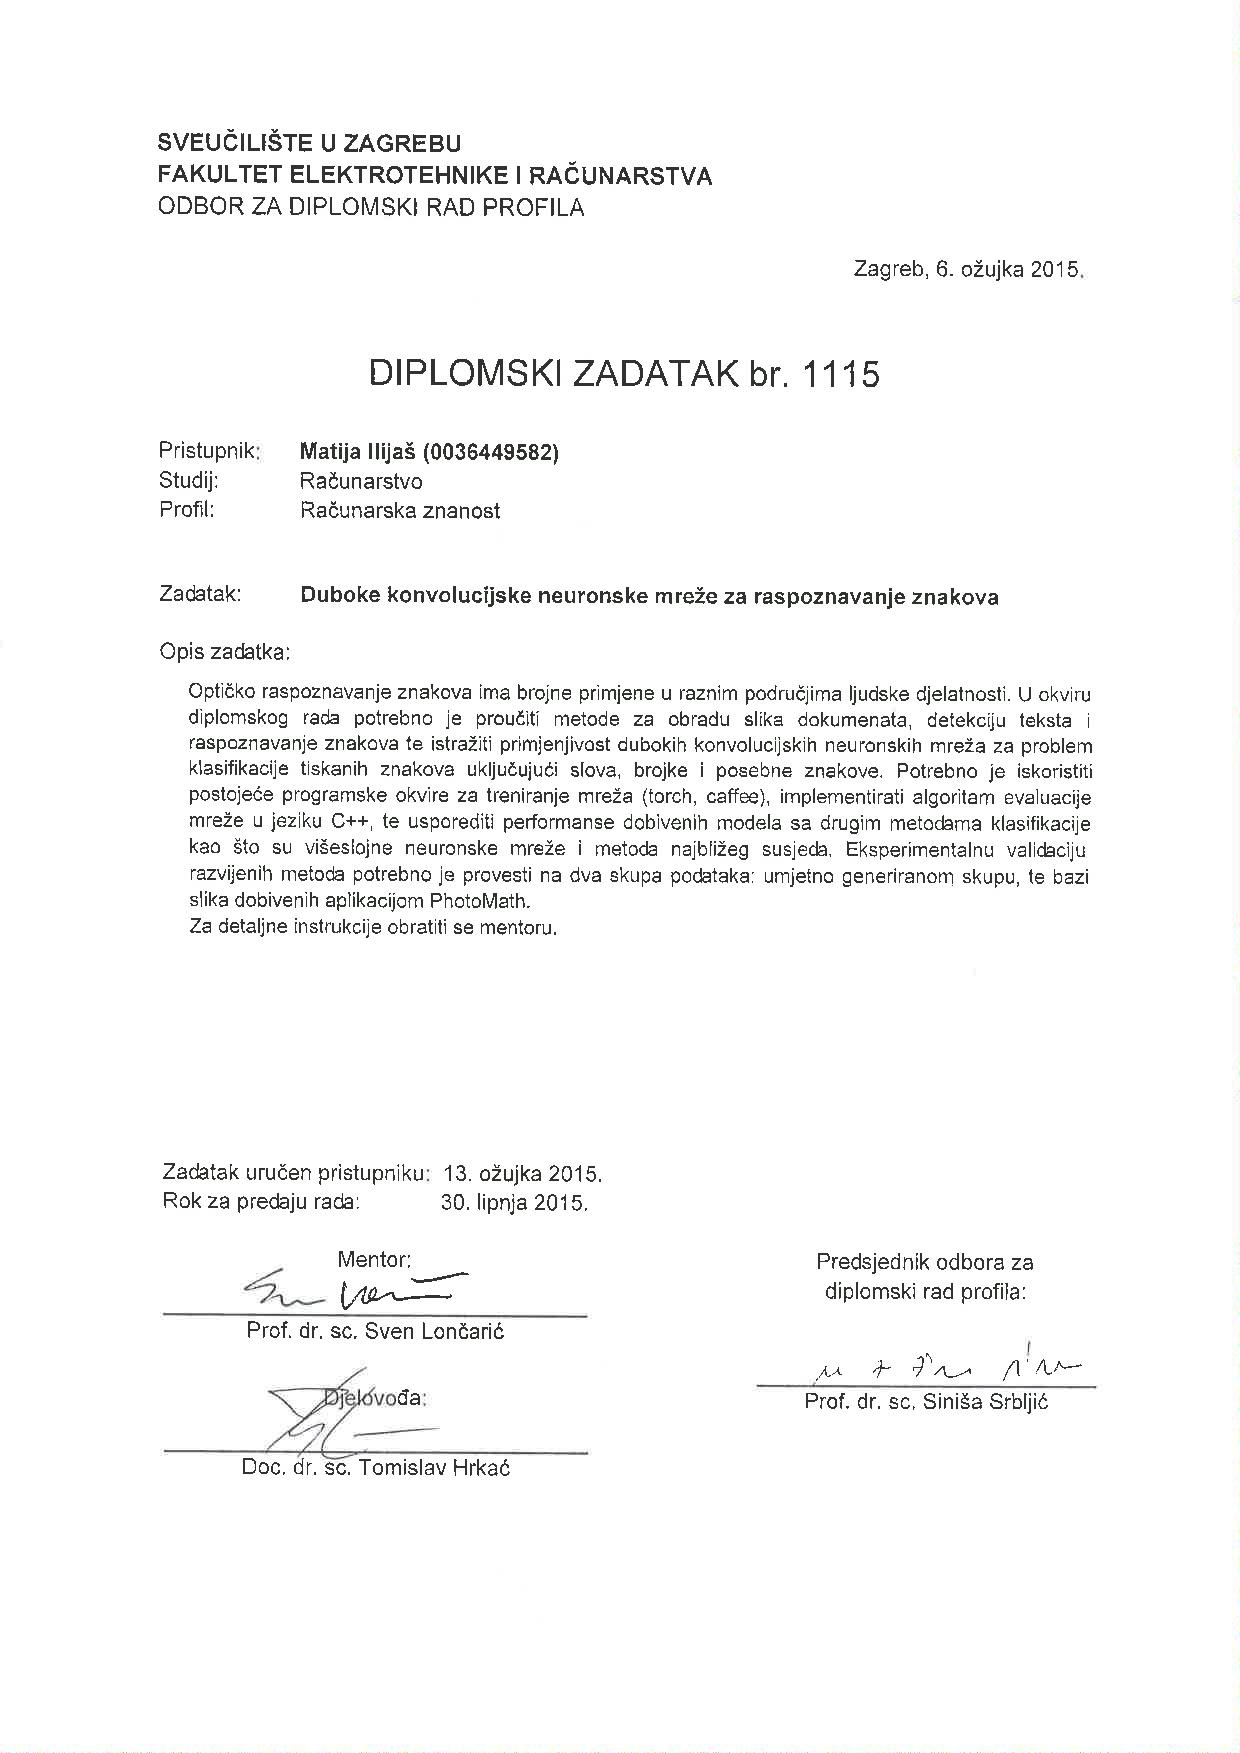
\includepdf[pages=-]{zadatak}

\tableofcontents

\chapter{Uvod}

Optičko prepoznavanje znakova  \engl{Optical Character Recognition – OCR} područje je istraživanja u računalnom vidu koje se bavi segmentacijom i klasifikacijom znakova sa slike. Prepoznavanje teksta sa slike ima vrlo široku primjenu u mnogim područjima ljudske djelatnosti. Jedna od trenutno najvećih primjena je arhiviranje i pretvorba dokumenata iz papirnatog oblika u digitalni oblik kako bi se mogli jednostavnije i brže pohranjivati i pretraživati. Razvijanjem mobilne tehnologije i njene primjene u svakodnevnom životu pojavljuju se nove izazovnije primjene optičkog prepoznavanja znakova koje zahtijevaju prepoznavanje teksta u prirodnim scenama. Tako se danas OCR algoritmi koriste za prepoznavanje podataka sa osobnih dokumenata i računa, prepoznavanje teksta za simultano prevođenje teksta, rješavanje matematičkih jednadžbi i mnoge druge primjene.

U strojnom učenju se u zadnjih nekoliko godina pojavilo novo obečavajuće područje istraživanja pod nazivom duboko učenje. Koncept dubokog učenja zasniva se na učenju korisnih prezentacija podataka povezanih u obliku hijerarhije, te je djelomično inspiriran vizualnim korteksom mozga sisavca. Zbog velike kompleksnosti modela dubokog učenja, te velike količine podataka potrebnih za učenje, istraživanja su u ovom području postala tek nedavno moguća uvođenjem specijaliziranih alata za brzo učenje na grafičkim karticama. Algoritmi dubokog učenja pokazali su jako dobre rezultate na problemima raspoznavanja uzoraka, posebice u području računalnog vida. Za problem klasifikacije na temelju slika razvijene su duboke konvolucijske neuronske mreže, također inspirirane vizualnim korteksom, koje su ostvarile najbolje rezultate na gotovo svim javno dostupnim skupovima za testiranje. Dodatni dokaz da duboko učenje u nekoj mjeri oponaša vizualni korteks su i nedavna istraživanja gdje su se značajke slike naučene dubokim učenjem pokazale sličnim onima u korteksu.

U ovom radu provedeno je istraživanje primjene dubokih konvolucijskih neuronskih mreža na problemu raspoznavanja znakova. U tu svrhu razvijen je sustav za učenje i testiranje različitih arhitektura standarnih neuronskih mreža te dubokih konvolucijskih neuronskih mreža. Podsustav za učenje implementiran je pomoću razvojnog alata za paralelno računanje na grafičkoj kartici kako bi postupak bio što brži. Dio sustava za testiranje razvijen je s ciljem detaljne analize rada naučenih modela, te jednostavne i pregledne usporedbe više različitih modela. 

Istraživanje je ostvareno uz dodatnu podršku tvrtke Microblink specijalizirane za razvoj tehnologija računalnog vida za mobilne uređaje. Za učenje i testiranje modela koriste se od tvrtke interni skupovi podataka, a prilikom testiranja provodi se analiza i njihovog internog klasifikatora. 
Rezultati su prikazani i komentirani sa ciljem pronalaska optimalne arhitekture modela za primjenu na mobilnom uređaju. Pritom je osim točnosti naučenih klasifikatora uzeta u obzir i njihova kompleksnost te prosječno trajanje klasifikacije.





\chapter{Optičko prepoznavanje znakova}

Proces optičkog prepoznavanja znakova provodi se u dva glavna koraka, segmentacije znakova iz slike i njihovog klasificiranja. U ovom radu provodi se istraživanje metoda klasifikacije, te se koristi već segmentirani skup znakova za učenje i testiranje klasifikatora. Stoga je u nastavku ovog poglavlja opisan drugi korak optičkog prepoznavanja znakova, njihovo klasificiranje.

Kao i kod svakog problema raspoznavanje uzoraka u računalnom vidu, transformacije ulaznih slika znakova nastale promjenjivim uvjetima okoline znatno otežavaju klasifikaciju. Promjenjiva pozadina znakova, moguća oštećenja i okluzije, te različita osvijetljenja prilikom slikanja mogu znatno promjeniti ulaznu sliku. Geometrijske transformacije posljedica su i različitih parametara kamere s kojom se slika, kao i pozicije kamere u odnosu na sliku prilikom slikanja.  
Kako bi se smanjio utjecaj transformacija ulazne slike, uobičajeni je postupak korištenje neke metode predprocesiranja prije slanja slike klasifikatoru.

\section{Predprocesiranje slike znaka}

Cilj predprocesiranja je proslijediti klasifikatoru sliku sa jasno definiranim područjem koje predstavlja znak. Često korišten postupak za dobivanje takve slike je metoda binarizacije, odnosno ograničavanje vrijednosti svih piksela slike na vrijednosti 0 ili 1. Tako dobivene binarne slike često imaju šum koji može otežati klasifikaciju, stoga se nakon binarizacije slika dodatno obrađuje morfološkim operacijama.

\subsection{Binariziranje slike}

Proces binarizacije uspoređuje svaku vrijednost piksela ulazne slike sa definiranim pragom, te ukoliko je njegova vrijednost veća dodjeljuje pikselu vrijednost 1, a u suprotnom vrijednost 0 (Izraz \ref{eq:thresh}). Postoji više metoda definiranja praga za pojedinačni piksel. Najjednostavnija metoda binarizacije koristi ručno određeni prag fiksne vrijednosti jednak za sve piksele. Ovako definiran prag je teško odrediti zbog promjenjivog intenziteta piksela pozadine i znaka, stoga naprednije metode računaju prag na temelju ulazne slike. 

\begin{equation}
\label{eq:thresh}
y(i,j) = \begin{cases}
1 & \text{ako } x(i,j) > prag \\
0 & \text{inače}\\
\end{cases}
\end{equation}

Jednostavniji pristup računanja praga na temelju slike koristi se svim vrijednostima piksela, te provodi binarizaciju piksela sa istim globalnim pragom. Ovako određen prag daje bolje rezultate od ručno određenog praga zbog bolje prilagođenosti pojedinačnoj slici, no zbog svoje fiksne vrijednosti za sve piksele nije robustan na lokalne promjene u kontrastu slike. 

Kako bi binarizacija bila robusna na promjene u osvijetljenju potrebno je određivati prag pojedinačno za svaki piksel u slici. Takav prag se zove adaptivni, te se računa na temelju lokalnog susjedstva piksela. Sama operacija računanja praga može biti jednostavni prosjek vrijednosti svih piksela u susjedstvu ili težinski prosjek koristeći na primjer 2D Gaussovu funkciju sa centrom na lokaciji piksela $(i,j)$:

\begin{equation}
\label{eq:gs}
w_{gauss}(i, j) = \frac{1}{\sigma \sqrt{2\pi }} \; exp \left (- \left( \frac{ \left (i - i_0 \right )^2}{ 2\sigma^2} + \frac{(j - j_0)^2}{ 2\sigma^2} \right ) \right )
\end{equation}

\hspace{2em}

Usporedba binariziranih slika globalnim i adaptivnim pragom može se vidjeti na Slici \ref{fig:adaglob}. Na područjima gdje razlika između piksela pozadine i znaka postaje vrlo mala, binarizacija globalnim pragom dala je lošije rezultate što je rezultiralo uklanjanjem ključne razlike između znaka 'G' i '6'.  

\begin{figure}[ht!]
\centering
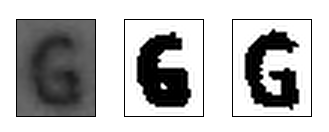
\includegraphics[width=10cm]{slike/thresholding_example.png}
\caption{Usporedba binarizacije sa globalnim i adaptivnim pragom}
\label{fig:adaglob}
\end{figure}


\subsection{Morfološke operacije}

Digitalnom morfologijom analiziraju se oblici digitalnih objekata. Slika se promatra u kontekstu teorije skupova te se predstavlja kao skup binarnih elemenata koji su grupirani u određene dvodimenzionalne strukture. Za obrađivanje binarnih slika tipično se koriste morfološke operacije dilatacije i erozije, te njihovih kombinacija, operacija zatvaranja i otvaranja. 

Dilatacija prolazi sa strukturnim elementom po slici i traži maksimalnu vrijednost piksela zahvaćenog dijela slike. Pronađenu maksimalnu vrijednost postavlja kao vrijednost svojeg središnjeg piksela, te na taj način proširuje svijetle regije piksela na slici.
Erozija, s druge strane, traži minimalnu vrijednost piksela te vrši isti postupak i proširuje tamne regije piksela. Binarna slika sadrži izdvojen znak u crnoj boji na bijeloj podlozi, odnosno predstavljena je tamnom regijom piksela okruženom svijetlim pikselima. Stoga su efekti ovih operatora obrnuti za potrebe obrade slika znakova.  

S obzirom da je u praksi teško znati kada je potrebna dilatacija a kada erozija, češće se koriste njihove kombinacije, otvaranje i zatvaranje.

\begin{equation}
\begin{gathered}
y(i,j) = \text{otvaranje(} x(i,j) \text{)} = \text{dilatacija(erozija(} x(i,j) \text{)}\\
y(i,j) = \text{zatvaranje(} x(i,j) \text{)} = \text{erozija(dilatacija(} x(i,j) \text{)}\\
\end{gathered}
\end{equation}

\hspace{2em}

Operacija otvaranja primjenjuje prvo eroziju pa dilataciju na slici, čime uklanja mala oštećenja na znakovima. Zatvaranje provodi prvo dilataciju slike a zatim eroziju, te time uklanja nepotrebni šum na slici. 



\begin{figure}[ht!]
\centering
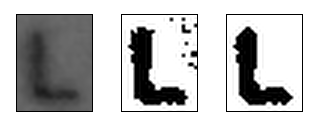
\includegraphics[width=10cm]{slike/closing_example.png}
\caption{Primjer uklanjanja šuma operacijom zatvaranja}
\end{figure}


\section{Klasifikacija slike znaka}

Kako bi odredili ASCII vrijednost znaka, potrebno je sliku znaka provesti kroz postupak klasifikacije. Standarni postupak razvijanja rješenja klasifikacije sastoji se od dva dijela, razvijanja kvalitetnih značajki koje olakšavaju klasifikaciju te razvijanja klasifikatora. 

Kvalitetne značajke koje olakšavaju klasifikaciju moraju zadovoljiti više uvjeta. Značajka prije svega treba biti diskriminantna, odnosno njena vrijednost mora biti različita za slike različitih znakova. Drugi uvjet je da vrijednost značajke ostaje ista za različite primjere slika istog znaka, odnosno da je robusna na moguće varijacije unutar jedne klase. Varijacije nastaju uslijed promjenjvih uvjeta okoline, a manifestiraju se najčešće kao geometrijske transformacije i lokalne promjene kontrasta. Stoga značajke trebaju biti invarijantne na promjene osvijetljenja i pomake kao što su translacija i rotacija. Značajke se mogu odrediti ručno na temelju promatranja podataka ili izravno iz skupa podataka metodama koje su opisane u kasnijim poglavljima ovog rada.

Općeniti problem učenja klasifikatora veliko je područje istraživanja, te će se opisati u kontekstu neuronskih mreža u kasnijim poglavljima. Važno je spomenuti svojstvo generalizacije kao glavno mjerilo dobre klasifikacije koje definira sposobnost klasifikatora da točno klasificira dotad neviđene primjere. Veliku ulogu u konačnim rezultatima klasifikatora imaju prethodno navedene metode određivanja značajki podataka, kao i sam skup podataka na kojima se klasifikator uči.


  

\chapter{Umjetne neuronske mreže}

Umjetna neuronska mreža \engl{Artificial Neural Network - ANN} algoritam je strojnog učenja inspiriran strukturom i funkcionalnošću ljudskog mozga. Zasniva se na paralelnoj obradi podataka, te vrlo dobro rješava probleme kod kojih postoji složena nelinearna veza ulaza i izlaza. Radi s velikim brojem parametara i varijabli, te može raditi s nejasnim podacima što ju čini robusnom na pogreške. Jedna od najčešćih primjena neuronskih mreža je u području raspoznavanja uzoraka, te se vrlo često koristi upravo za raspoznavanje znakova.

 

\section{Arhitektura neuronske mreže}

Neuronska mreža se sastoji od tri vrste sloja: ulaznog, izlaznog, te skrivenog koji povezuje prethodna dva. Čvorišta, tzv. neuroni, skrivenog sloja povezani su težinskim vezama s ulaznim i izlaznim neuronima. Standarna arhitektura neuronske mreže je potpuno povezana i aciklička što znači da su svi neuroni iz susjednih slojeva međusobno povezani te da nema ciklusa u mreži između neurona. 

\begin{figure}[ht!]
\centering
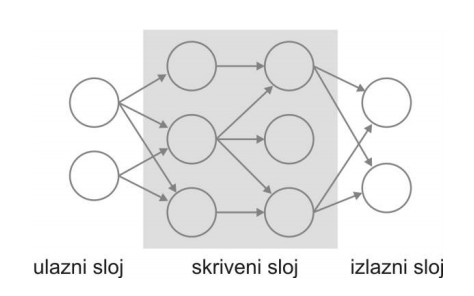
\includegraphics[width=10cm]{slike/neural_architecture.png}
\caption{Primjer jednostavne arhitekture neuronske mreže}
\end{figure}

Umjetni neuron je matematička funkcija inspirirana funkcionalnošću biološkog neurona koja radi težinsku sumu svojih ulaza a zatim primjenjuje svoju prijenosnu funkciju na izlazu \cite{neuron1943pitts}. Ako ulaze neurona definiramo sa vektorom $x$ duljine $m$ i njegove težine jednim redom matrice težina $w$, tada se izlaz neurona $k$ može definirati izrazom:

\begin{equation}
y_k = f \left (\sum\limits_{j=0}^m w_{kj} x_j \right )          
\end{equation}

\hspace{2em}

gdje je $f$ prijenosna funkcija neurona. Kako bi mreža mogla predstaviti visoko nelinearni odnos između njenog ulaza i izlaza, prijenosna funkcija njenih neurona mora biti nelinearna funkcija. Najčešće korištena prijenosna funkcija je sigmoidalna funkcija koja se koristi zbog svojeg blažeg prijenosa od obične funkcije s fiksnim pragom i svoje derivabilnosti, te je poseban slučaj logističke funkcije definirane izrazom:

\begin{equation}
f(x) = \frac{1}{1 + e^{-x}}
\end{equation}

\hspace{2em}

\section{Učenje neuronskih mreža}

Dvije su faze rada umjetnih neuronskih mreža, učenje i eksploatacija. Učenje je iterativan postupak predočavanja ulaznih primjera i očekivanog izlaza pri čemu dolazi do postupnog prilagođavanja težina veza neurona. Nakon što se težine skrivenog sloja prilagode postupkom učenja, eksploatacijom neuronske mreže može se za do tad neviđeni ulazni primjer dobiti pripadajući izlaz.

Jedna neuronska mreža sa svojim težinama može se gledati kao nelinearna funkcija sa više varijabli, te se njeno učenje može opisati kao traženje minimuma te funkcije s obzirom na grešku klasifikacije. Ako se uzme u obzir da izlazni sloj može sadržavati više neurona, pogreška se može definirati izrazom:

\begin{equation}
E(\vec{w}) = \frac{1}{2} \sum\limits_{d \in D} \sum\limits_{k \in izlazi} (t_{kd} - o_{kd})^2
\end{equation}

\hspace{2em}

pri čemu je $t_{kd}$ tražena izlazna vrijednost i $o_{kd}$  izlazna vrijednost dobivena mrežom za $k$-ti neuron na primjeru podatka za učenje $d$ \cite{cupic2008neuro}. Metoda minimiziranja ove pogreške zove se gradijentni spust \engl{Gradient descent}, a algoritam koji implementira tu metodu za učenje neuronske mreže zove se algoritam propagacije greške unatrag \engl{Backpropagation algorithm} \cite{backProp}. Radi gradijentne metode prijenosna funkcija neurona mora biti derivabilna kako bi se mogli računati gradijenti, što vrijedi za ranije spomenutu sigmoidalnu funkciju.

Glavna mjera uspješnosti neuronske mreže u klasifikaciji je njena sposobnost generalizacije, odnosno koliko dobro može klasificirati primjere koji nisu korišteni prilikom njenog učenja. Stoga se za potrebe učenja neuronskh mreža podatci dijele na dva (a nekad i tri) skupa: skup za učenje, skup za testiranje i ponekad skup za dodatnu evaluaciju. Kada je greška klasifikacije velika na testnom skupu a mala na skupu za učenje kažemo da je mreža pretjerano prilagođena skupu za učenje \engl{Overfitting}. Kako bi se dobila mreža sa najboljom sposobnošću generalizacije, postupak učenja se zaustavlja kada se greška mreže na testnom skupu prestane smanjivati. Pojednostavljeni prikaz jednog takvog postupka može se vidjeti na Slici \ref{fig:generalization}. 

\begin{figure}[ht!]
\centering
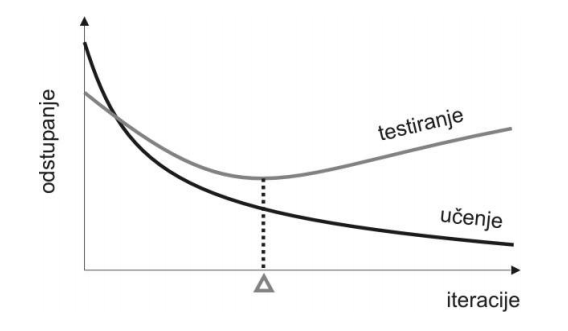
\includegraphics[width=10cm]{slike/generalization.png}
\caption{Prikaz greške klasifikacije prilikom učenja mreže}
\label{fig:generalization}
\end{figure}


\chapter{Duboko učenje}

Duboko učenje se u zadnjih nekoliko godina pojavilo kao novo obečavajuće područje strojnog učenja. Iako je sama ideja prezentirana u radovima Kunihika Fukushime \cite{fukushima1980deep} i Yanna Lecuna \cite{lecun1989zipcode} prije gotovo 30 godina, duboko učenje je postalo predmetom istraživanja relativno nedavno. Razlog tome su bila tada nedovoljno snažna računala za učenje velikih modela karakterističnih za taj pristup. Koncept dubokog učenja zasniva se na učenju korisnih prezentacija podataka povezanih u obliku hijerarhije. Ideja je djelomično inspirirana vizualnim korteksom mozga sisavaca koji se sastoji od niza procesirajućih elemenata koji obrađuju vizualni podražaj. Dokaz da duboko učenje u nekoj mjeri oponaša vizualni korteks su i nedavna istraživanja gdje su se naučene značajke pokazale slične onima u korteksu. Glavna karakteristika algoritama dubokog učenja je velik broj slojeva kroz koje ulazni podatak mora proći do izlaza, gdje se prvi dio prolaza može zamisliti kao formiranje hijerarhijskog prikaza podatka, a drugi kao proces klasifikacije. Time jedan algoritam dubokog učenja ustvari preuzima zadatak izvlačenja korisnih značajki iz podataka uz sami zadatak klasifikacije. Kod učenja takvog algoritma cijeli se postupak uči na temelju podataka, te se time gubi potreba za ručnim definiranjem značajki podataka. 

\section{Hijerarhijski prikaz podataka}

Slika se može klasifikatoru prikazati na mnogo načina, od kojih je najjednostavniji vektor vrijednosti intenziteta piksela. Apstraktniji prikaz bio bi recimo skup rubova na slici, a još apstraktniji skup različitih oblika. Neki prikazi olakšavaju klasifikatoru proces učenja, a različiti problemi klasifikacije zahtijevaju razvijanje različitih prikaza odnosno značajki ulaznih podataka. Stoga  se tradicionalno razvijanje rješenja problema klasifikacije sastoji od dva dijela, razvijanja kvalitetnih značajki koje olakšavaju učenje te razvijanja klasifikatora. 

Uobičajeni proces razvoja kvalitetnih značajki podrazumijeva promatranje svojstva ulaznih podataka te naglašavanje onih koja su maksimalno diskriminantna. Napredak u točnosti klasifikacije većim dijelom se ostvaruje razvijanjem boljih značajki, tako je na primjer značajni napredak u prepoznavanju čovjeka ostvaren razvijanjem značajki pomoću histograma orijentiranih gradijenata \engl{Histogram of Oriented Gradients - HoG} \cite{dalal2005hog}. Histogrami su dobro opisivali lokalne oblike te u isto vrijeme bili u velikoj mjeri invarijantni na  promjene osvijetljenja i geometrijske transformacije. 

No negativna strana postupka razvijanja značajki koje se baziraju na ljudskom promatranju podataka je gubitak informacija koje čovjek nije u stanju vidjeti. Kako bi se koristile sve informacije iz podataka, potrebne su metode koje određuju diskriminantne značajke izravno iz skupa podataka. Među popularnijim metodama tog tipa su metoda linearne diskriminantne analize \engl{Linear Discriminant Analysis - LDA} te metoda glavnih komponenata \engl{Principal Component Analysis - PCA}. Linearna diskriminantna analiza pronalazi prikaz podataka koji maksimalno diskriminira podatke različitih klasa, dok metoda glavnih komponenata prikazuje podatke kao linearnu kombinaciju linearno nekoreliranih varijabli koje imaju najveću varijancu.

\begin{figure}[ht!]
\centering
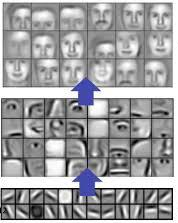
\includegraphics[height=9cm]{slike/feature_hierarchy.png}
\caption{Hijerarhija značajki ljudskog lica naučena dubokim učenjem}
\label{fig:hierarchy}
\end{figure}

Istraživanja vizualnog korteksa mozga sisavaca pokazala su da vizualni podražaj prolazi kroz hijerarhiju više procesirajućih slojeva gdje svaki dodatni sloj predstavlja dodatnu razinu apstrakcije značajki.  Značajke dobivene prethodno navedenim metodama predstavljaju jednu razinu apstrakcije, te se mogu zamisliti kao imitacija najnižeg sloja vizualnog korteksa. Ideja dubokog učenja je naučiti cijelu hijerarhiju značajki, odnosno imitirati i više slojeve vizualnog korteksa. Primjer jedne takve hijerarhije značajki ljudskog lica naučene dubokim učenjem prikazan je na Slici \ref{fig:hierarchy}.


\section{Učenje dubokih mreža}

Kao što je ranije spomenuto ideja dubokog učenja je naučiti hijerarhiju značajki iz podataka. S obzirom da to zahtijeva nekoliko dodatnih slojeva mreže, kompleksnost dubokih modela značajno je veća od standarnih. Poznato je da količina potrebnih podataka za kvalitetno učenje modela raste proporcionalno sa brojem njegovih slobodnih parametara. Stoga je za učenje dubokih mreža potrebno značajno više podataka nego kod učenja standarnih klasifikatora. Nedovoljna količina podataka za učenje, te nedovoljno jaka računala za učenje tako velikih modela, razlog su zašto duboko učenje nije zaživjelo 1980-ih godina kada je prvi put predstavljeno kao ideja. Dolazak specijaliziranih razvojnih alata za brzo učenje mreža na grafičkim karticama, kao i sve veća količina dostupnih podataka za učenje, omogućili su da duboko učenje u zadnjih nekoliko godina pokaže svoj potencijal na raznim problemima strojnog učenja.

Jedna od velikih prednosti dubokog učenja je što uz metode nadziranog učenja ima razvijene i metode nenadziranog učenja. U ovom radu koristi se isključivo nadzirano učenje zbog dostupnosti velike količine označenih podataka. U nastavku ovog poglavlja opisana je metoda nenadziranog učenja, a metoda nadziranog učenja opisana je u idućem poglavlju kao uvod u duboke konvolucijske mreže.

Sve veća količina podataka postaje dostupna za učenje, no velikim dijelom radi se o neoznačenim podatcima. Kako bi se i ti podatci iskoristili potrebne su metode nenadziranog učenja. Kao što je ranije spomenuto, duboki modeli predstavljaju hijerarhiju značajki podataka, a jednu razinu apstrakcije moguće je postići metodama poput metode glavnih komponenata. Stoga se u teoriji postavlja pitanje da li uzastopnim primjenjivanjem metode glavnih komponenata možemo dobiti traženu hijerarhiju. Odgovor na to pitanje je da ne možemo, a razlog tome je linearnost te metode. Uzastopnom linearnom transformacijom konačno se uvijek dobiva linearna transformacija, što onemogućuje stvaranje željene hijerarhije. Iz tog razloga koriste se dvije metode sa dodanom nelinearnošću, autoenkoderi \engl{Autoencoders} i ograničeni Boltzmann strojevi \engl{Restricted Boltzmann Machines - RBM} \cite{bengio2009auto}\cite{hinton2006rbm}. U sklopu ovog rada opisati će se autoenkoderi, jednostavnija i intuitivnija metoda od dvije navedene.

Autoenkoder je jednostavna troslojna neuronska mreža kod koje su izlazni neuroni izravno povezani sa ulaznim neuronima. Ulazni i izlazni sloj imaju jednak broj neurona, a u srednjem sloju ima ih manje. Kao posljedica toga prolaskom podataka kroz mrežu događaju se dvije radnje, enkodiranje i dekodiranje. 

\begin{figure}[ht!]
\centering
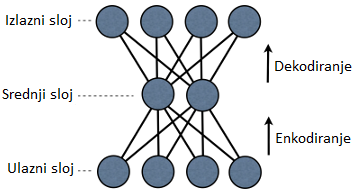
\includegraphics[width=9cm]{slike/autoencoder.png}
\caption{Prikaz rada autoenkodera}
\end{figure}

Enkodiranje se može definirati kao postupak preslikavanja ulaznog vektora $x$ u vektor elemenata skrivenog sloja $y$ izrazom:

\begin{equation}
y = f \left (Wx + b \right)          
\end{equation}


gdje je $f$ nelinearna prijenosna funkcija (npr. sigmoidalna), a $W$ matrica težina autoenkodera. Zato što je broj neurona srednjeg sloja manji od broja elemenata ulaznog sloja, ulazni vektor se kompresira, odnosno podatak se u srednjem sloju prikazuje pomoću apstraktnijih značajki. Nakon toga vrši se dekompresija, odnosno dekodiranje, kako bi se na temelju značajki iz srednjeg sloja rekonstruirao ulazni vektor. Postupak dekodiranja vektora značajki srednjeg sloja $y$ u vektor rekonstrukcijskog izlaznog sloja $z$ definiran je izrazom: 

\begin{equation}
z = f \left (W'y + b' \right)          
\end{equation}

gdje se $W'$ može definirati kao $W^{T}$, transpozicija matrice težina $W$. U tom slučaju autoenkoder ima takozvano svojstvo povezanih težina \engl{Tied weights}, što smanjuje konačan broj parametara koje je potrebno naučiti. Vrijednosti izlaznog vektora zatim se uspoređuju sa onima ulaznog vektora kako bi se dobila informacija o kvaliteti rekonstrukcije, odnosno koliko dobro značajke iz srednjeg sloja predstavljaju ulazni podatak. Rekonstrukcijska greška može se računati na mnogo načina, od kojih je jedan od jednostavnijih korištenje funkcije kvadratne greške:

\begin{equation}
E(xz) = (x-z)^2          
\end{equation}

Proces učenja autoenkodera sastoji se od iterativnog enkodiranja i dekodiranja ulaznih podataka za učenje te korigiranja njegovih težina na temelju greške u rekonstrukciji. Rezultat je autoenkoder sa težinama koje čine elemente njegovog srednjeg sloja apstraktnim značajkama koje dobro opisuju prezentirane podatke. S obzirom da autoenkoder radi nelinearnu transformaciju nad ulaznim podatcima, možemo ostvariti hijerarhiju apstraktnih značajki slijednim povezivanjem više autoenkodera. Učenje se provodi iterativno, odnosno prvi autoenkoder uči se na temelju ulaznih podataka, a svaki idući na temelju naučenih značajki svojeg prethodnika. 

\begin{figure}[ht!]	
\centering
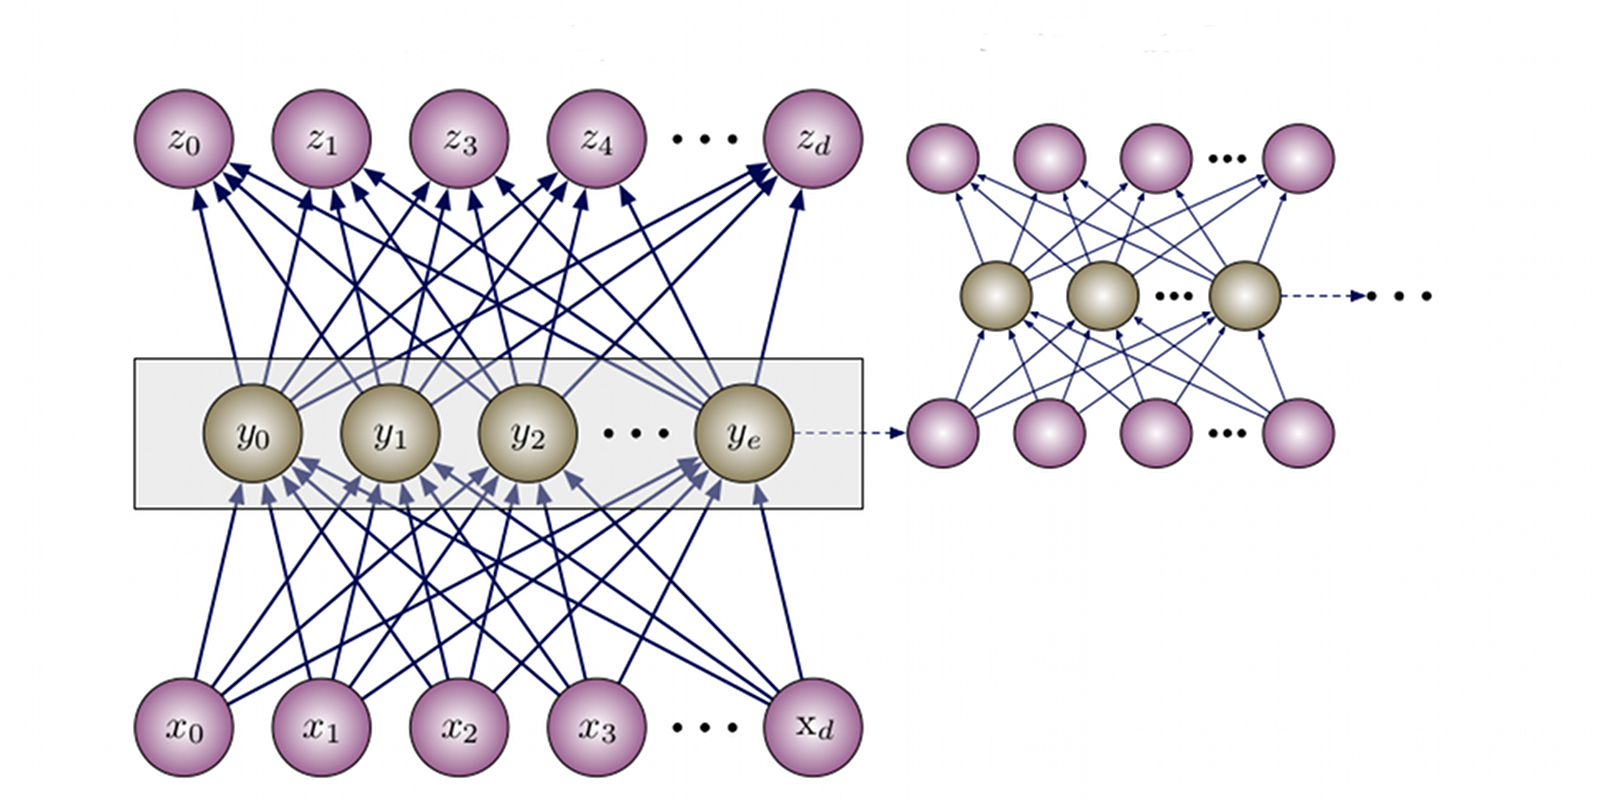
\includegraphics[width=16cm]{slike/stacked_autoencoders.jpg}
\caption{Prikaz iterativnog učenja slijeda autoenkodera}
\end{figure}

Ovako dobivena mreža naučena je isključivo na neoznačenim podatcima te predstavlja hijerarhiju značajki podataka bez mogućnosti klasifikacije. Konačni klasifikator dobiva se dodavanjem jedne manje mreže koja na ulaz prima značajke zadnjeg autoenkodera a na izlaz vraća klase zadanog problema. Tako povezana mreža autoenkodera i mreža za klasifikaciju zatim se uče na označenim podatcima kao jedna velika mreža.


\chapter{Duboke konvolucijske neuronske mreže}

U prethodnom poglavlju opisana je metoda nenadziranog učenja koja može naučiti hijerarhiju značajki koristeći se neoznačenim podatcima, a zatim naučiti klasificirati pomoću manjeg skupa označenih podataka. Ovaj pristup je praktičan u većini problemskih domena zbog male količine dostupnih označenih podataka za učenje. No u praksi se pokazalo da za određene probleme, gdje ima dovoljno označenih podataka, najbolje rezultate daju metode nadziranog učenja. Problemska domena ovog rada ima dostupnu veliku količinu označenih podataka, te su svi modeli učeni metodama nadziranog učenja.

Kao i kod nenadziranog učenja, konačni model koji se uči sastoji se od dijela za formiranje hijerarhije značajki i dijela za klasifikaciju, no nadzirano učenje je proces koji se provodi u jednom koraku i na jednom skupu podataka. Sam postupak učenja ne razlikuje se od standarnog učenja neuronske mreže metodom gradijentnog spusta.

Istraživanja vizualnog korteksa pokazala su da njegovi procesirajući elementi reagiraju na male lokalne podražaje unutar vizualnog polja, funkcionirajući kao lokalni receptori. Glavna karakteristika prirodnih slika je njihova lokalna prostorna korelacija, pa je logično da se vizualni korteks prilagodio traženju lokalnih značajki.
Klasične neuronske mreže sa potpuno povezanim slojevima ne iskorištavaju ovo korisno svojstvo, što je potaknulo Yanna Lecuna 1989. godine da razvije model konvolucijske neuronske mreže \cite{lecun1998lenet}. Razvijena mreža oponaša lokalne receptore vizualnog korteksa sa svojim lokalnim prostornim filterima ostvarenim konvolucijom (Izraz \ref{eq:convfilt}).

\begin{equation}
y(m,n) = x(m,n)  \ast h(m,n) = \sum\limits_{j=-\infty}^{\infty} \sum\limits_{i=-\infty}^{\infty} x(i,j) h(m-i,n-j)  
\label{eq:convfilt}
\end{equation}

\section{Lokalni prostorni filteri}

Konvolucijom ostvareni filteri omogućuju provođenje kompleksnih operacija jednostavnom promjenom konvolucijske jezgre. Tako bi na primjer upotrebom Gaussianove jezgre dobili za rezultat zamućenje slike, a upotrebom Sobelove jezgre \cite{sobel1968operator} naglašene rubove na slici. Ručno definiranje konvolucijskih jezgri upravo odgovara ranije spomenutom ručnom određivanju značajki u standarnom postupku razvijanja klasifikatora. Cilj konvolucijske neuronske mreže je naučiti konvolucijske jezgre specifične za dane podatke, što odgovara ranije spomenutom učenju značajki iz podataka.

U dubokoj konvolucijskoj mreži prvih nekoliko slojeva zaduženih za izgradnju hijerarhije značajki je konvolucijsko. Uloga prvog sloja konvolucije je jasna s obzirom da odgovara standarnom filtriranju slike sa nekom konvolucijskom jezgrom. Viši slojevi konvolucije nemaju doticaja sa ulaznom slikom, već formiraju apstraktnije lokalne značajke od značajki prethodnog sloja. Na primjer u problemu detekcije čovjeka prvi sloj konvolucije razvio bi lokalne detektore rubova na slici, sloj iznad njega formirao bi lokalne oblike koristeći se sa rubovima iz prvog sloja, a sloj za razinu više bi koristio lokalne oblike za formiranje detektora dijelova tijela čovjeka. Jednom kada mreža ima detektore značajki koje opisuju prisutnost glavnih dijelova objekta, u ovom slučaju čovjeka, problem klasifikacije postaje znatno jednostavniji.

\begin{figure}[ht!]
\centering
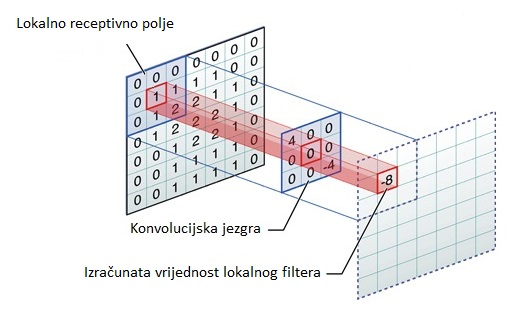
\includegraphics[width=14cm]{slike/kernel_convolution.jpg}
\caption{Primjer računanja vrijednosti lokalnog prostornog filtera}
\end{figure}

\section{Dijeljenje težina}

Jednom naučeni lokalni filteri mogu prepoznati neku značajku podataka, no nepoznato je gdje se ta značajka nalazi u prostoru. Kako bi razvili lokalne filtere invarijantne na poziciju u prostoru, potrebno je za svaki filter imati skup njegovih inačica koje pokrivaju sve moguće podprostore. Takav skup zovemo mapa značajki  \engl{Feature maps} , a glavna karakteristika takve mape je dijeljenje težina između svih elemenata skupa. Svaki element konvolucijskog sloja prikazuje se tada kao matrica koja sadrži vrijednosti odziva  pripadajućeg filtera za svaku poziciju u prostoru. Dijeljenje težina na višoj razini apstrakcije prikazano je na Slici \ref{fig:sharedWeights}, gdje je važno primjetiti da konvolucija nakon prvog sloja postaje trodimenzionalna zbog uvođenja mape značajki koja je dvodimenzionalni prikaz elementa konvolucijskog sloja.

\begin{figure}[ht!]
\centering
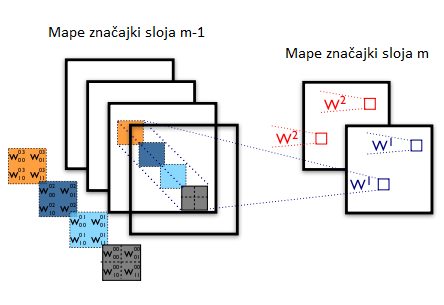
\includegraphics[width=12cm]{slike/shared_weights.png}
\caption{Prikaz dijeljenja težina na višoj razini apstrakcije}
\label{fig:sharedWeights}
\end{figure}

Za učenje mreža sa dijeljenim težinama još uvijek se može koristiti metoda gradijentnog spusta, ali uz malu preinaku. Gradijent dijeljene težine računa se kao suma gradijenata svih parametara koji se dijele. 
Osim što ostvaruje prostornu invarijantnost lokalnih filtera, dijeljenje težina znatno doprinosi i procesu učenja konvolucijske mreže. Dijeljenjem težina između parametara  mreže smanjujemo ukupan broj slobodnih parametara koje je potrebno naučiti, što smanjuje trajanje učenja. No ono što je još važnije, smanjenjem broja slobodnih parametara poboljšava se sposobnost generalizacije mreže stavljanjem dodatnog ograničenja na njenu kompleksnost.  

\section{Lokalno udruživanje}

Još jedan važan koncept dubokih konvolucijskih mreža je lokalno udruživanje \engl{Pooling}, koje se može definirati kao oblik nelinearnog poduzorkovanja. U praksi se najviše koristi inačica maksimalnog lokalnog udruživanja \engl{Max pooling} koja za poduzorkovanje koristi operaciju traženja maksimuma. 
Postupak maksimalnog lokalnog udruživanja na slici sastoji se od dijeljenja slike na nepreklapajuće podprozore fiksne veličine, te uzimanja maksimalne vrijednosti svakog podprozora za rezultat. Dobivena slika za podprozore veličine 2x2 bila bi u tom slučaju dvostruko manja od originalne slike, sa vrijednostima svih maksimalnih elemenata podprozora. 
Maksimalno lokalno udruživanje se u dubokim konvolucijskim mrežama ne primjenjuje na ulaznoj slici, već kao dodatni sloj nakon svakog sloja konvolucije. Time ova metoda postaje korisna na dva načina: eliminira vrijednosti koje nisu maksimalne što smanjuje količinu računanja u višim slojevima, te ostvaruje jedan oblik invarijantnosti na translaciju. Invarijantnost proizlazi iz činjenice da se uzimanjem maksimalne vrijednosti nekog podprozora prepoznaje odziv lokalnog filtera na bilo kojoj lokaciji unutar podprozora, odnosno dopušta se mali pomak naučenih značajki u prostoru.


\begin{figure}[ht!]
\centering
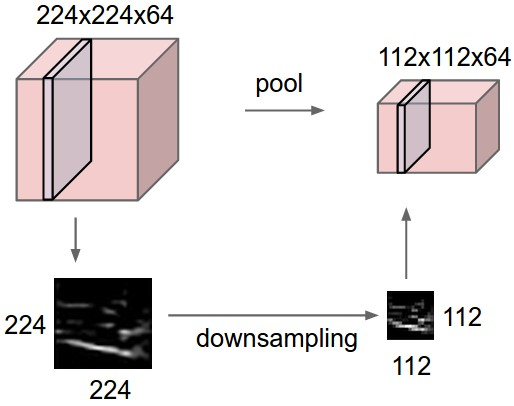
\includegraphics[width=11cm]{slike/max_pooling.jpeg}
\caption{Primjer lokalnog udruživanja na 10 mapa značajki}
\end{figure}


\section{Ispravljena linearna jedinica}

Ono što razlikuje neuronske mreže od linearnih klasifikatora su dodane prijenosne funkcije za postizanje nelinearnosti. U standarnoj potpuno povezanoj neuronskoj mreži svaki element sadrži prijenosnu funkciju, najčešće sigmoidalnog tipa. Dodavanje nelinearnosti u dubokoj konvolucijskoj mreži postiže se dodavanjem sloja koji na svaku vrijednost prijašnjeg sloja primjenjuje prijenosnu funkciju. 

Primjenom sigmoidalne prijenosne funkcije (Izraz \ref{eq:sigcomp}) kod učenja duboke arhitekture pojavljuje se problem nestajućeg gradijenta \engl{Vanishing gradient problem} \cite{hochreiter2001vanish}. Zbog svojstva sigmoidalne funkcije da ograničava vrijednosti na mali izlazni interval, vrijednosti gradijenata postaju izrazito male ukoliko se prosljeđuju kroz veliki broj slojeva, što onemogućuje kvalitetno učenje. Rješenje ovog problema prvi je osmislio Yoshua Bengio primjenom ispravljene linearne jedinice \engl{Rectified Linear Unit - ReLU} koja ne ograničava vrijednosti veće od nule \cite{bengio2011relu}. Ispravljena prijenosna funkcija definirana je operacijom maksimuma, što ju čini izrazito jednostavnom za računanje (Izraz \ref{eq:reccomp}).

\begin{equation}
f(x) = \frac{1}{1 + e^{-x}}
\label{eq:sigcomp}
\end{equation}

\begin{equation}
f(x) = \text{max}(x, 0)
\label{eq:reccomp}          
\end{equation}

\hspace{2em}

 Osim što se rješava problem nestajućeg gradijenta, postiže se i efekt raspršene aktivacije, odnosno u prosjeku se samo pola elemenata aktivira svakim prolazom kroz mrežu što pospješuje sposobnost generalizacije.  

\begin{figure}[ht!]
\centering
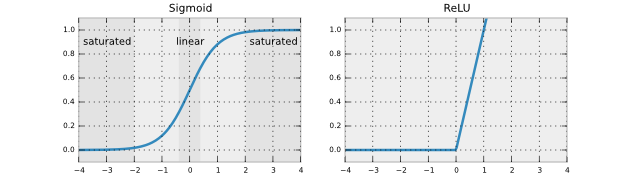
\includegraphics[width=15cm]{slike/sigmoid_relu.png}
\caption{Usporedba sigmoidalne funkcije i ispravljene linearne jedinice}
\end{figure}

\newpage

\section{Konačni model}

Kao što je ranije spomenuto, konačni model duboke konvolucijske mreže sastoji se od dijela za formiranje hijerarhije značajki i dijela za klasifikaciju. Prvi dio modela ostvaren je slojevima koji implementiraju ranije spomenute koncepte dubokih konvolucijskih mreža, a drugi standardnim potpuno povezanima slojevima. 

Nakon svakog sloja konvolucije dodaje se sloj maksimalnog lokalnog udruživanja, a zatim sloj ispravljenih linearnih jedinica za postizanje nelinarnosti. Primjer jednog takvog konačnog modela prikazan je na Slici \ref{fig:cnnmodel}, uz pretpostavku da se nakon svakog sloja lokalnog udruživanja primjenjuje prijenosna funkcija.

\begin{figure}[ht!]
\centering
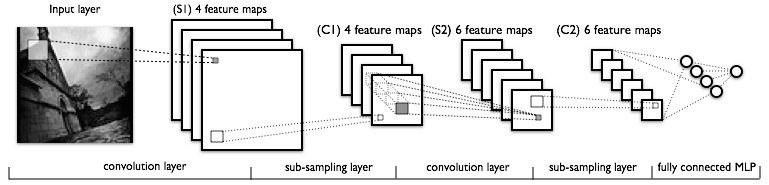
\includegraphics[width=15cm]{slike/convnet.jpg}
\caption{Primjer modela duboke konvolucijske neuronske mreže}
\label{fig:cnnmodel}
\end{figure}

Odabir arhitekture dubokih konvolucijskih mreža dodatno je otežan u odnosu na standarne neuronske mreže. Osim standarnih hiperparametara koji određuju broj slojeva i broj elemenata po sloju mreže, za duboku konvolucijsku arhitekturu potrebno je odrediti veličine lokalnih prostornih filtera i filtera maksimalnog lokalnog udruživanja. Veličine lokalnih filtera ponajprije ovise o veličine ulazne slike, te je cilj odrediti veličinu kojom će se kvalitetno formirati apstrakcije značajki po slojevima mreže. Veličine filtera maksimalnog lokalnog udruživanja uobičajeno su male zbog gubljenja velike količine podataka kod većih filtera. Također je važno uzeti u obzir da se veličine mapa značajki smanjuju nakon svakog sloja konvolucije i lokalnog udruživanja, što se u praksi kompenzira dodavanjem većeg broj mapa u višim slojevima.



\chapter{Implementacija}

U sklopu ovog rada razvijen je sustav za učenje i testiranje različitih arhitektura neuronskih mreža. Prilikom razvijanja takvog sustava bilo je važno zadovoljiti dva glavna uvjeta: brzo učenje kompleksnih arhitektura na velikoj količini podataka te detaljna analiza rada naučenih mreža. Iz tog razloga sustav je podijeljen na dva podsustava razvijena sa zasebnim alatima. Podsustav zadužen za učenje implementiran je u razvojnom alatu Torch koji omogućuje paralelno izvođenje procesa učenja na grafičkoj kartici \cite{collobert2011torch}. Podsustav koji provodi analizu rada naučenih mreža implementiran je u jeziku C++ korištenjem OpenCV biblioteke \cite{bradski2000opencv}, a za pokretanje Torch modela u tom okruženju koristi se C++ biblioteka JTorch koju je razvio Jonathan Tompson \cite{tompson2013jtorch}.

Kako bi se dobio dodatni uvid u rad naučenih neuronskih mreža napravljena je prilagodba C++ implementacije Torch modela OCR sustavu tvrtke Microblink. Time je omogućeno korištenje naučenih modela kao klasifikatora u Microblink mobilnim aplikacijama te dodatna analiza primjenom na mobilnom uređaju.

\section{Sustav za učenje}

Kako bi cijeli proces istraživanja različitih arhitektura mreža i podataka bio što efikasniji, potrebno je prije svega imati brz sustav za učenje. Učenje velikih arhitektura na velikoj količini podataka može trajati tjednima, pa i mjesecima, sekvencijalnim računanjem na standarnom procesoru računala. Stoga je tek pojavom specijaliziranih biblioteka koje omogućuju optimizirano paralelno računanje na grafičkoj kartici postalo moguće provoditi istraživanje u području dubokog učenja. 
Osim brzine učenja, važna je i jednostavnost definiranja parametara mreže koja se uči, kao i parametara samog procesa učenja. Kod implementacije ovog rada odabran je razvojni alat Torch zbog svoje jednostavnosti i brzine, ali i podrške velikih kompanija kao što su Facebook i Google, koje nerijetko dijele korisne implementacije sa zajednicom. 

\subsection{Torch razvojni alat}

Prilikom odabira razvojnog alata uzeti su u obzir i alati Caffe i Theano \cite{jia2014caffe}\cite{bergstra2010theano}. Možda najpopularniji alat za duboko učenje Caffe ima izrazito jednostavno sučelje za odabir parametara mreže i procesa učenja, no kao posljedica toga teško je raditi promjene u postojećoj implementaciji u svrhu istraživanja ili razvoja. Theano s druge strane pruža puno manju razinu apstrakcije te ostavlja mogućnost lake izmjene većine implementacije, no postaje nepraktičan kod česte upotrebe standarnih algoritama.
Torch je po razini apstrakcije negdje između prethodno navedenih alata, dovoljno je niske apstrakcije za laku izmjenu implementacije kod razvoja i istraživanja, ali ima i sučelje za standarne algoritme koje ga čini praktičnim. 

Brzina samog izvođenja procesa učenja na grafičkim karticama velikim dijelom ovisi o pozadinskoj implementaciji paralelnog računanja koja je za sve navedene alate otprilike podjednako brza, te se toliko često mijenja da nema smisla uspoređivati njihove brzine. S druge strane, važan faktor kod odabira alata je podrška akademske zajednice i industrije s obzirom da o tome ovisi koliko brzo se razvijaju implementacije novih koncepata. Torch ima implementaciju za većinu novih koncepata u dubokom učenju zbog podrške kompanija kao što su Google, Facebook i Twitter.  Tako je primjerice implementirana relativno nova metoda izbacivanja \engl{Dropout}\cite{hinton2014dropout} za regularizaciju prilikom učenja mreže te ispravljena linearna jedinica \engl{Rectified Linear Unit - ReLU}, funkcija prijelaza koja je pokazale bolje rezultate od standardne sigmoidalne funkcije u nedavnim istraživanjima.

Sama implementacija Torcha podijeljena je na dva dijela. Sve računske operacije na grafičkoj kartici napisane su kao C/CUDA implementacija za maksimalnu brzinu, dok je ostatak funkcionalnosti implementiran u skriptnom jeziku LuaJIT za lakše korištenje alata.  

\subsection{Definiranje arhitekture}
	
Neuronska mreža je u Torch alatu definirana kao model koji se sastoji od sekvencijalno povezanih slojeva koji vrše različite računske operacije.
Tako je na primjer standarna dvoslojna neuronska mreža definirana kao sekvencijalni niz koji prvo linearno množi ulazni vektor sa težinama prvog sloja, zatim primjenjuje prijenosnu sigmoidalnu funkciju na svim elementima prvog sloja, te konačno linearno množi vektor elemenata prvog sloja sa težinama drugog sloja kako bi se dobile izlazne vrijednosti mreže. Jedan takav Torch model prikazan je na Slici \ref{fig:nnmodel}.

\begin{figure}[ht!]
\centering
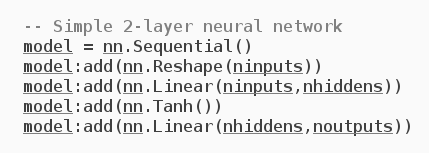
\includegraphics[width=10cm]{slike/nn_model.png}
\caption{Definiranje Torch modela dvoslojne neuronske mreže}
\label{fig:nnmodel}
\end{figure}
\FloatBarrier

Za definiranje duboke konvolucijske mreže u Torchu potrebno je dodatno koristiti slojeve za prostornu konvoluciju, maksimalno lokalno udruživanje i ispravljene linearne jedinice. Primjer definiranja jednog dubokog konvolucijskog modela prikazan je na Slici \ref{fig:cnntorch}.

\begin{figure}[ht!]
\centering
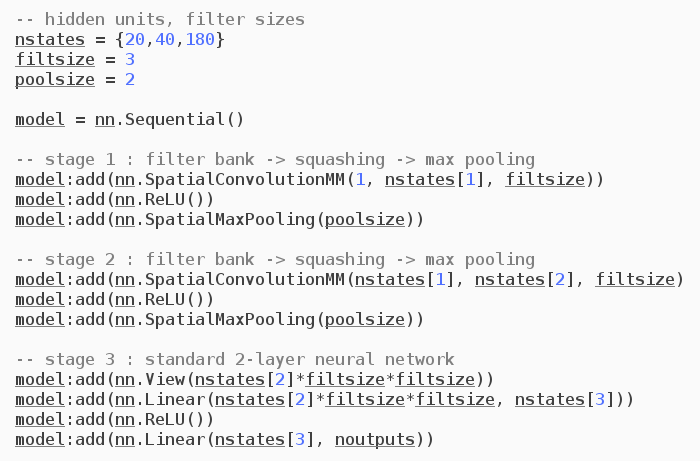
\includegraphics[width=16cm]{slike/cnn_model.png}
\caption{Definiranje Torch modela duboke konvolucijske neuronske mreže}
\label{fig:cnntorch}
\end{figure}

\newpage

\section{Sustav za testiranje}

Detaljna analiza rada naučenih mreža ključna je za pronalaženje optimalne arhitekture. Mjera optimalnosti nekog modela općenito se može definirati kao omjer njegove točnosti klasifikacije i njegove kompleksnosti. Ovisno o području primjene postoje određena ograničenja i prioriteti za različite karakteristike modela. U ovom radu razvijen je sustav koji analizira naučene mreže u dovoljno detalja da bi se donosili kvalitetni zaključci o njihovoj primjenjivosti. Osim analize pojedinih modela omogućeno je i simultano analiziranje više modela za što lakšu usporedbu njihovih pojedinih karakteristika.  

\subsection{Matrica greške klasifikacije}

Testiranjem klasifikatora na skupu podataka u konačnici se dobivaju dvije oznake klasa za svaki podatak. Jedna oznaka je ručno određena te uvijek predstavlja točnu klasu podatka, dok drugu dobivamo kao rezultat klasifikatora koji se testira. Standarna mjera točnosti klasifikatora koristi se dobivenim oznakama samo za informaciju o tome da li oznaka klasifikatora odgovara označenoj oznaci, te vraća kao informaciju ukupni postotak točno klasificiranih podataka. Promatranjem klasa oznaka koje klasifikator vraća u slučaju krive klasifikacije može se dobiti bolji uvid u rad analiziranog modela. 

\begin{figure}[ht!]
\centering
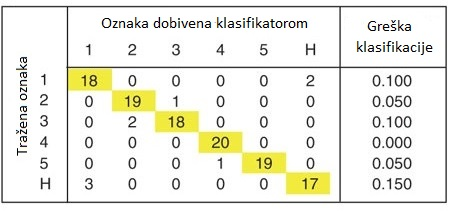
\includegraphics[width=12cm]{slike/confusion_matrix.jpg}
\caption{Primjer matrice greške klasifikacije}
\end{figure}

Matrica greške klasifikacije definirana je redovima koji predstavljaju ručne oznake klasa, te stupcima koji predstavljaju oznake dobivene klasifikatorom. Matrica se generira brojanjem uređenih parova ručne oznake i oznake klasifikatora, odnosno tražene i dobivene oznake. Tako bi na primjer potpuno točan klasifikator generirao matricu sa vrijednostima nula na svim mjestima osim na glavnoj dijagonali matrice gdje su tražene i dobivene oznake jednake.
Ovakav prikaz greške klasifikacije omogućuje uvid u točnost klasifikatora za pojedine klase, kao i informaciju o klasama koje se često međusobno zamjenjuju.



\subsection{Prosječno trajanje klasifikacije}

Kako bi se donio zaključak o primjenjivosti nekog modela potrebno je poznavati i mjeru njegove kompleksnosti. Sustav za testiranje računa za svaku arhitekturu ukupan broj računskih operacija potrebnih za klasifikaciju jedne slike. Kod standarnih potpuno povezanih mreža taj broj odgovara ukupnom broju veza između neurona, dok se kod kovolucijskih arhitektura prilikom računanja tog broja moraju uzeti u obzir veličine filtera i mjere njihovog preklapanja. 

Kompleksnost modela se može definirati i brojem slobodnih parametara, koji se koristi i za procjenu sposobnosti generalizacije klasifikatora. Kod potpuno povezanih mreža broj slobodnih parametara jednak je broju računskih operacija. Kod dubokih konvolucijskih arhitektura taj je broj manji od broja računskih operacija zbog ranije opisane metode dijeljenja težina lokalnih filtera. 

Iako se pomoću broja računskih operacija može aproksimirati prosječno trajanje klasifikacije, sustav za testiranje provodi i empirijsko mjerenje. Testiranjem klasifikatora na skupu podataka bilježi se vrijeme potrebno da klasifikator odredi ulaznoj slici oznaku, što nam omogućuje računanje prosječnog trajanja klasifikacije.

\subsection{Simultano analiziranje više modela}

Osim analize pojedinih modela, sustav za testiranje omogućuje i simultano analiziranje više modela s ciljem njihove lakše usporedbe. Kod simultanog analiziranja prikazuju se sve ranije navedene informacije za svaki pojedini model, uz dodatak tabličnih prikaza pojedinih karakteristika svih modela. 

Kako bi rezultati bili što pregledniji, nakon analize svih modela generiraju se dva tablična prikaza. Prva tablica omogućuje lako uspoređivanje točnosti klasifikatora po pojedinim klasama i njihove ukupne točnosti. Druga tablica prikazuje prosječno trajanje klasifikacije za svaki analizirani model. 

Kod problema klasifikacije slika analizu znatno olakšava mogućnost vizualne provjere podataka. Vrlo često se može donijeti neki zaključak o slabostima klasifikatora promatranjem slika krivo klasificiranih primjera. Sustav za testiranje sprema za svaki analizirani model krivo klasificirane slike u zasebne datoteke ovisno o krivo određenoj klasi.

\section{Prilagodba Microblink OCR sustavu}

Istraživanje u ovom radu ostvareno je uz dodatnu podršku tvrtke Microblink koja razvija rješenja za mobilne uređaje u području računalnog vida. Njihovo rješenje sastoji se od vlastitog OCR sustava optimiziranog za rad na mobilnom uređaju, te implementacija raznih mobilnih aplikacija koje primjenjuju taj sustav. Neke od implementacija su aplikacije za plaćanje računa, izvlačenja informacija iz osobnih dokumenata, pa čak i rješavanje matematičkih jednadžbi. 

Microblink OCR sustav sastoji se od dva glavna dijela, podsustava za segmentaciju znakova sa slike, te podsustava za klasifikaciju tih znakova. U ovom radu analizirani su modeli neuronskih mreža za klasifikaciju znakova, te su ulazni skupovi podataka već segmentirani znakovi iz slike. Stoga kako bi se naučeni modeli mogli pokretati na mobilnom uređaju napravljena je prilagodba C++ implementacije Torch modela sučelju Microblink podsustava za klasifikaciju.

Sa implementiranom prilagodbom Microblink sustavu moguće je koristiti bilo koji naučeni Torch model kao klasifikator u bilo kojoj Microblink mobilnoj aplikaciji. Time je omogućena dodatna analiza rada modela iz njegove izravne primjene na mobilnom uređaju. Korištenjem aplikacija može se dobiti uvid u točnost i brzinu klasifikacije u raznim uvjetima i na različitim mobilnim uređajima.  


\chapter{Rezultati}

Cilj ovog rada bio je analizirati rad dubokih konvolucijskih mreža na problemu raspoznavanja znakova te ih usporediti sa standarnim neuronskim mrežama. Modeli su učeni i testirani na internim skupovima podataka tvrtke Microblink, a prilikom testiranja provedena je analiza i njihovog internog klasifikatora. 

Istraživanje je provedeno na problemu raspoznavanja znakova na osobnim iskaznicama, takozvanim strojno čitljivim područjima \engl{Machine Readable Zone - MRZ}. MRZ podatci imaju 37 klasa znakova fonta ocrb, te obuhvaćaju znamenke, velika slova i znak manje. U ovom radu koriste se dva skupa takvih podataka za učenje i testiranje klasifikatora. Prvi skup zove se sintetizirani skup, a dobiven je slikanjem printanih imitacija osobnih iskaznica. Sastoji se od 450 tisuća označenih slika znakova te je slikan sa više različitih modela mobitela u raznim uvjetima osvijetljenja. Drugi skup dobiven je slikanjem pravih osobnih iskaznica u različitim uvjetima, te sadrži oko 12 tisuća ručno označenih slika znakova. Za potrebe učenja i testiranja sintetizirani skup je podijeljen na 300 tisuća slika za učenje i 150 tisuća za testiranje modela, a ručno označeni skup koristi se za dodatno testiranje sposobnosti generalizacije modela.



\section{Utjecaj predprocesiranja podataka}


U ranijim poglavljima spomenuta je uobičajena praksa predprocesiranja slika znakova prije njihovog klasificiranja. Promjenjivi uvjeti okoline rezultiraju raznim transformacijama originalne slike koje otežavaju njenu klasifikaciju, stoga je logično primjenjivati metode ublažavanja posljedica tih transformacija. Takve metode najčešće su neki oblik operacije binarizacije, različite po načinu na koji se definira njihov prag. Jedna takva metoda koja uzima u obzir lokalne promjene osvijetljenja je metoda adaptivnog praga opisana ranije u radu.

Metode predprocesiranja razvijene su sa ciljem naglašavanja korisnih informacija, te odbacivanjem onih nepotrebnih. Mana ovog pristupa je što se odluka o korisnosti informacija donosi pomoću ručno razvijenih metoda zasnovanih na ljudskom promatranju podataka, zbog čega dolazi do gubitka korisnih informacija koje čovjek nije u stanju vidjeti. Kako bi se koristile sve informacije iz podataka, potrebne su metode koje pronalaze korisne informacije izravno iz skupa podataka. Takve metode razvijaju se u području dubokog učenja gdje se na temelju skupa podataka uči cijela hijerarhija značajki i klasifikator u jednom procesu učenja. Posljedice promjenjivih uvjeta okoline se tada rješavaju na način da se procesom učenja na velikoj količini različitih oblika podataka razvije kvalitetna hijerarhija značajki otporna na nastale transformacije.

U ovom radu provedeno je istraživanje kako bi se analizirao utjecaj predprocesiranja podataka na točnost klasifikatora. Korištena je duboka konvolucijska mreža sa 10 mapa značajki u prvom i 20 mapa značajki u drugom konvolucijskom sloju. Testiranje je provedeno na slikama dimenzija 18 piksela u 3 različita oblika: predprocesiranim metodom adaptivnog praga, predprocesiranim internom metodom tvrtke Microblink, te originalnim slikama bez predprocesiranja.
 
\hspace{2em}
\begin{table}[ht!]
\begin{center}
\centering
    \begin{tabular}{ | c| c| c|c |}
    \hline
    Skup podataka & Adaptivni prag & Microblink interni & Bez predprocesiranja \\ \hline
    Sintetizirani & 98.29\% & 97.87\%  & 99.57\% \\ \hline
    Ručno označeni & 96.35\% & 97.66\% & 99.21\% \\  
    \hline
    \end{tabular}
\end{center}
\caption{Rezultati istraživanja utjecaja predprocesiranja podataka}
\label{tab:preproc}
\end{table}

Dobiveni rezultati su općenito lošiji za ručno označeni testni skup, što je logično s obzirom da su mreže učene na sintetiziranom skupu koji je dobiven slikanjem printanih imitacija osobnih iskaznica. Rezultati mreže učene na originalnim podacima bez predprocesiranja pokazuju da mreža dobro generalizira s obzirom da su postotci točnosti klasifikacija na oba testna skupa vrlo visoki. Interna metoda tvrtke Microblink pokazala je lošije rezultate na oba testna skupa, no bolje od metode adaptivnog praga koja je vrlo loše generalizirala na ručnom testnom skupu.   

\begin{figure}[ht!]
\centering
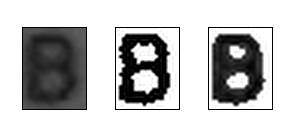
\includegraphics[width=13cm]{slike/preprocessing_comparison.png}
\caption{Primjer predprocesiranja slike adaptivnim pragom i Microblink metodom}
\label{fig:preproc}
\end{figure}

Analizom krivo klasificiranih primjera za mreže koje se koriste predprocesiranim podatcima može se dobiti bolji uvid u probleme ovog pristupa. Jedan takav primjer može se vidjeti na Slici \ref{fig:preproc}. Prikazana je originalna slika slova 'B' lijevo, slika dobivena predprocesiranjem adaptivnim pragom u sredini, te rezultat primjene Microblink metode predprocesiranja desno. Veliki broj krivo klasificiranih slika za mreže sa predprocesiranim podatcima rezultat je zamjene slova 'B' i znamenke '8'. Za razlikovanje ove dvije klase jedna dobro naučena mreža koristiti će se razlikom u zaobljenosti njihovih znakova. Na Slici \ref{fig:preproc} može se vidjeti da metode predprocesiranja binariziranjem krivo označavaju neke dijelove slike, čime znak poprima zaobljenost karakterističnu za znamenku '8'.




\section{Pronalaženje optimalne arhitekture mreže}

Glavna mjera kvalitete naučenog modela je njegova sposobnost generalizacije, odnosno koliko dobro klasificira dotad neviđene primjere. Odabir prave arhitekture modela ključan je za dobru generalizaciju, stoga je u ovom radu proveden postupak pronalaženja optimalne arhitekture. Ovaj postupak se još naziva i selekcija modela, a zasniva se na testiranju više arhitektura različitih kompleksnosti. Prilikom odabira optimalne arhitekture postupno se povećava kompleksnost modela, te se promatra njegova točnost na skupovima podataka za testiranje. 

Selekcija modela napravljena je za standarne neuronske mreže i duboke konvolucijske neuronske mreže kako bi se u konačnici mogli usporediti rezultati njihovih najboljih arhitektura.

\subsection{Standarne neuronske mreže}

Dodavanje slojeva neuronskoj mreži u teoriji omogućuje razvijanje hijerarhije značajki koja robusnije predstavlja objekt klasifikacije. U svrhu što boljeg razumijevanja utjecaja dubine arhitekture i njenog tipa (standarni ili konvolucijski) na uspješnost klasifikacije,  provedeno je istraživanje i nad dubokim standarnim neuronskim mrežama. Analiziran je rad 5 arhitektura različitih dubina, od plitke dvoslojne mreže do duboke mreže sa šest slojeva. Rezultati su prikazani uzlazno s obzirom na njihovu kompleksnost na Slici \ref{graf:nncomplex}. 

\begin{figure}[ht!]
\begin{center}
    % GNUPLOT: LaTeX picture with Postscript
\begingroup
  \makeatletter
  \providecommand\color[2][]{%
    \GenericError{(gnuplot) \space\space\space\@spaces}{%
      Package color not loaded in conjunction with
      terminal option `colourtext'%
    }{See the gnuplot documentation for explanation.%
    }{Either use 'blacktext' in gnuplot or load the package
      color.sty in LaTeX.}%
    \renewcommand\color[2][]{}%
  }%
  \providecommand\includegraphics[2][]{%
    \GenericError{(gnuplot) \space\space\space\@spaces}{%
      Package graphicx or graphics not loaded%
    }{See the gnuplot documentation for explanation.%
    }{The gnuplot epslatex terminal needs graphicx.sty or graphics.sty.}%
    \renewcommand\includegraphics[2][]{}%
  }%
  \providecommand\rotatebox[2]{#2}%
  \@ifundefined{ifGPcolor}{%
    \newif\ifGPcolor
    \GPcolorfalse
  }{}%
  \@ifundefined{ifGPblacktext}{%
    \newif\ifGPblacktext
    \GPblacktexttrue
  }{}%
  % define a \g@addto@macro without @ in the name:
  \let\gplgaddtomacro\g@addto@macro
  % define empty templates for all commands taking text:
  \gdef\gplbacktext{}%
  \gdef\gplfronttext{}%
  \makeatother
  \ifGPblacktext
    % no textcolor at all
    \def\colorrgb#1{}%
    \def\colorgray#1{}%
  \else
    % gray or color?
    \ifGPcolor
      \def\colorrgb#1{\color[rgb]{#1}}%
      \def\colorgray#1{\color[gray]{#1}}%
      \expandafter\def\csname LTw\endcsname{\color{white}}%
      \expandafter\def\csname LTb\endcsname{\color{black}}%
      \expandafter\def\csname LTa\endcsname{\color{black}}%
      \expandafter\def\csname LT0\endcsname{\color[rgb]{1,0,0}}%
      \expandafter\def\csname LT1\endcsname{\color[rgb]{0,1,0}}%
      \expandafter\def\csname LT2\endcsname{\color[rgb]{0,0,1}}%
      \expandafter\def\csname LT3\endcsname{\color[rgb]{1,0,1}}%
      \expandafter\def\csname LT4\endcsname{\color[rgb]{0,1,1}}%
      \expandafter\def\csname LT5\endcsname{\color[rgb]{1,1,0}}%
      \expandafter\def\csname LT6\endcsname{\color[rgb]{0,0,0}}%
      \expandafter\def\csname LT7\endcsname{\color[rgb]{1,0.3,0}}%
      \expandafter\def\csname LT8\endcsname{\color[rgb]{0.5,0.5,0.5}}%
    \else
      % gray
      \def\colorrgb#1{\color{black}}%
      \def\colorgray#1{\color[gray]{#1}}%
      \expandafter\def\csname LTw\endcsname{\color{white}}%
      \expandafter\def\csname LTb\endcsname{\color{black}}%
      \expandafter\def\csname LTa\endcsname{\color{black}}%
      \expandafter\def\csname LT0\endcsname{\color{black}}%
      \expandafter\def\csname LT1\endcsname{\color{black}}%
      \expandafter\def\csname LT2\endcsname{\color{black}}%
      \expandafter\def\csname LT3\endcsname{\color{black}}%
      \expandafter\def\csname LT4\endcsname{\color{black}}%
      \expandafter\def\csname LT5\endcsname{\color{black}}%
      \expandafter\def\csname LT6\endcsname{\color{black}}%
      \expandafter\def\csname LT7\endcsname{\color{black}}%
      \expandafter\def\csname LT8\endcsname{\color{black}}%
    \fi
  \fi
    \setlength{\unitlength}{0.0500bp}%
    \ifx\gptboxheight\undefined%
      \newlength{\gptboxheight}%
      \newlength{\gptboxwidth}%
      \newsavebox{\gptboxtext}%
    \fi%
    \setlength{\fboxrule}{0.5pt}%
    \setlength{\fboxsep}{1pt}%
\begin{picture}(7200.00,5040.00)%
    \gplgaddtomacro\gplbacktext{%
      \colorrgb{0.50,0.50,0.50}%
      \put(814,704){\makebox(0,0)[r]{\strut{}$92$}}%
      \colorrgb{0.50,0.50,0.50}%
      \put(814,1213){\makebox(0,0)[r]{\strut{}$93$}}%
      \colorrgb{0.50,0.50,0.50}%
      \put(814,1722){\makebox(0,0)[r]{\strut{}$94$}}%
      \colorrgb{0.50,0.50,0.50}%
      \put(814,2231){\makebox(0,0)[r]{\strut{}$95$}}%
      \colorrgb{0.50,0.50,0.50}%
      \put(814,2740){\makebox(0,0)[r]{\strut{}$96$}}%
      \colorrgb{0.50,0.50,0.50}%
      \put(814,3248){\makebox(0,0)[r]{\strut{}$97$}}%
      \colorrgb{0.50,0.50,0.50}%
      \put(814,3757){\makebox(0,0)[r]{\strut{}$98$}}%
      \colorrgb{0.50,0.50,0.50}%
      \put(814,4266){\makebox(0,0)[r]{\strut{}$99$}}%
      \colorrgb{0.50,0.50,0.50}%
      \put(814,4775){\makebox(0,0)[r]{\strut{}$100$}}%
      \colorrgb{0.50,0.50,0.50}%
      \put(1922,484){\makebox(0,0){\strut{}2}}%
      \colorrgb{0.50,0.50,0.50}%
      \put(2898,484){\makebox(0,0){\strut{}3}}%
      \colorrgb{0.50,0.50,0.50}%
      \put(3875,484){\makebox(0,0){\strut{}4}}%
      \colorrgb{0.50,0.50,0.50}%
      \put(4851,484){\makebox(0,0){\strut{}5}}%
      \colorrgb{0.50,0.50,0.50}%
      \put(5827,484){\makebox(0,0){\strut{}6}}%
      \colorrgb{0.50,0.50,0.50}%
      \put(6803,484){\makebox(0,0){\strut{}}}%
    }%
    \gplgaddtomacro\gplfronttext{%
      \csname LTb\endcsname%
      \put(176,2739){\rotatebox{-270}{\makebox(0,0){\strut{}Točnost klasifikacije (\%)}}}%
      \put(3874,154){\makebox(0,0){\strut{}Broj slojeva mreže}}%
      \csname LTb\endcsname%
      \put(5816,1097){\makebox(0,0)[r]{\strut{}Synth450}}%
      \csname LTb\endcsname%
      \put(5816,877){\makebox(0,0)[r]{\strut{}Manual}}%
    }%
    \gplbacktext
    \put(0,0){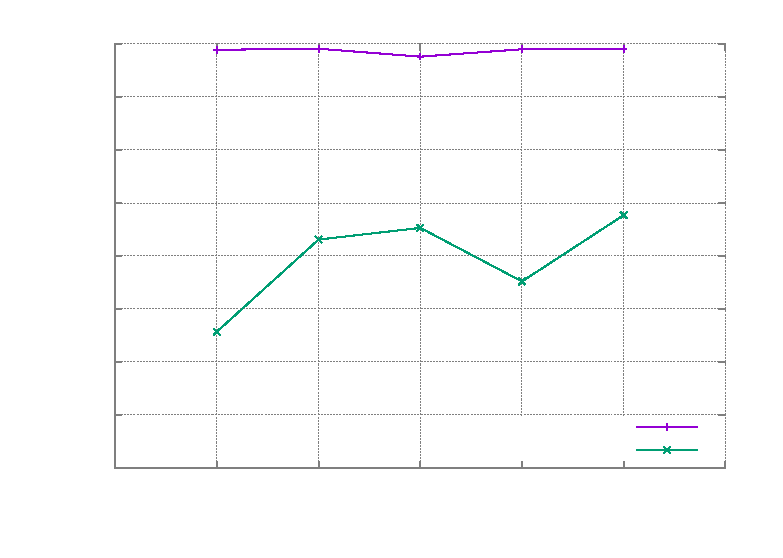
\includegraphics{grafovi/nn_complexity}}%
    \gplfronttext
  \end{picture}%
\endgroup

    \caption{Usporedba 5 arhitektura neuronskih mreža različitih dubina}
\label{graf:nncomplex}
\end{center}
\end{figure}

Dobiveni rezultati pokazuju značajnu razliku u točnosti klasifikacije između dva testna skupa za sve arhitekture. Prilikom testiranja ustanovljeno je da svi klasifikatori vrlo dobro generaliziraju na testnom sintetiziranom skupu iako on nije korišten za njihovo učenje. Razlog tome mogu biti kontrolirani uvjeti u kojima je sintetizirani skup generiran, te jednolikost printanih imitacija kartica. Rezultati na ručno označenom setu lošiji su nego na sintetiziranom za sve arhitekture te nam daju bolji uvid u sposobnost generalizacije standarnih neuronskih mreža.

Utjecaj dubine arhitekture, odnosno broja slojeva mreže, nije vidljiv na rezultatima na sintetiziranom testnom skupu zbog već vrlo visokog postotka točnosti klasifikacije dvoslojne mreže. Na ručno označenom skupu vidljivi su bolji rezultati prilikom dodavanja jednog sloja dubine dvoslojnoj arhitekturi, no dodatno dodavanje slojeva ne pokazuje značajno i konzistentno bolje rezultate. Stoga je optimalna arhitektura standarnih neuronskih mreža ona sa tri sloja neurona.

\subsection{Konvolucijske neuronske mreže}

Kod definiranja arhitekture konvolucijskih mreža postoje određena ograničenja prilikom odabira njenih parametara. S obzirom da se ulazna slika postepeno smanjuje u dimenzijama zbog primjene konvolucijske jezgre i lokalnog udruživanja, broj slojeva mreže je ograničen. U ovom radu koriste se relativno male ulazne slike dimenzija 18 piksela te lokalni filteri dimenzija 3 piksela, stoga mreže mogu imati najviše dva konvolucijska sloja. Analizirano je 7 arhitektura sa različitim brojem mapa značajki u svakom konvolucijskom sloju, te su prikazani rezultati s obzirom na njihovu kompleksnost na Slici \ref{graf:cnncomplex}.

\begin{figure}[ht!]
\begin{center}
    % GNUPLOT: LaTeX picture with Postscript
\begingroup
  \makeatletter
  \providecommand\color[2][]{%
    \GenericError{(gnuplot) \space\space\space\@spaces}{%
      Package color not loaded in conjunction with
      terminal option `colourtext'%
    }{See the gnuplot documentation for explanation.%
    }{Either use 'blacktext' in gnuplot or load the package
      color.sty in LaTeX.}%
    \renewcommand\color[2][]{}%
  }%
  \providecommand\includegraphics[2][]{%
    \GenericError{(gnuplot) \space\space\space\@spaces}{%
      Package graphicx or graphics not loaded%
    }{See the gnuplot documentation for explanation.%
    }{The gnuplot epslatex terminal needs graphicx.sty or graphics.sty.}%
    \renewcommand\includegraphics[2][]{}%
  }%
  \providecommand\rotatebox[2]{#2}%
  \@ifundefined{ifGPcolor}{%
    \newif\ifGPcolor
    \GPcolorfalse
  }{}%
  \@ifundefined{ifGPblacktext}{%
    \newif\ifGPblacktext
    \GPblacktexttrue
  }{}%
  % define a \g@addto@macro without @ in the name:
  \let\gplgaddtomacro\g@addto@macro
  % define empty templates for all commands taking text:
  \gdef\gplbacktext{}%
  \gdef\gplfronttext{}%
  \makeatother
  \ifGPblacktext
    % no textcolor at all
    \def\colorrgb#1{}%
    \def\colorgray#1{}%
  \else
    % gray or color?
    \ifGPcolor
      \def\colorrgb#1{\color[rgb]{#1}}%
      \def\colorgray#1{\color[gray]{#1}}%
      \expandafter\def\csname LTw\endcsname{\color{white}}%
      \expandafter\def\csname LTb\endcsname{\color{black}}%
      \expandafter\def\csname LTa\endcsname{\color{black}}%
      \expandafter\def\csname LT0\endcsname{\color[rgb]{1,0,0}}%
      \expandafter\def\csname LT1\endcsname{\color[rgb]{0,1,0}}%
      \expandafter\def\csname LT2\endcsname{\color[rgb]{0,0,1}}%
      \expandafter\def\csname LT3\endcsname{\color[rgb]{1,0,1}}%
      \expandafter\def\csname LT4\endcsname{\color[rgb]{0,1,1}}%
      \expandafter\def\csname LT5\endcsname{\color[rgb]{1,1,0}}%
      \expandafter\def\csname LT6\endcsname{\color[rgb]{0,0,0}}%
      \expandafter\def\csname LT7\endcsname{\color[rgb]{1,0.3,0}}%
      \expandafter\def\csname LT8\endcsname{\color[rgb]{0.5,0.5,0.5}}%
    \else
      % gray
      \def\colorrgb#1{\color{black}}%
      \def\colorgray#1{\color[gray]{#1}}%
      \expandafter\def\csname LTw\endcsname{\color{white}}%
      \expandafter\def\csname LTb\endcsname{\color{black}}%
      \expandafter\def\csname LTa\endcsname{\color{black}}%
      \expandafter\def\csname LT0\endcsname{\color{black}}%
      \expandafter\def\csname LT1\endcsname{\color{black}}%
      \expandafter\def\csname LT2\endcsname{\color{black}}%
      \expandafter\def\csname LT3\endcsname{\color{black}}%
      \expandafter\def\csname LT4\endcsname{\color{black}}%
      \expandafter\def\csname LT5\endcsname{\color{black}}%
      \expandafter\def\csname LT6\endcsname{\color{black}}%
      \expandafter\def\csname LT7\endcsname{\color{black}}%
      \expandafter\def\csname LT8\endcsname{\color{black}}%
    \fi
  \fi
    \setlength{\unitlength}{0.0500bp}%
    \ifx\gptboxheight\undefined%
      \newlength{\gptboxheight}%
      \newlength{\gptboxwidth}%
      \newsavebox{\gptboxtext}%
    \fi%
    \setlength{\fboxrule}{0.5pt}%
    \setlength{\fboxsep}{1pt}%
\begin{picture}(7200.00,5040.00)%
    \gplgaddtomacro\gplbacktext{%
      \colorrgb{0.50,0.50,0.50}%
      \put(814,704){\makebox(0,0)[r]{\strut{}$92$}}%
      \colorrgb{0.50,0.50,0.50}%
      \put(814,1213){\makebox(0,0)[r]{\strut{}$93$}}%
      \colorrgb{0.50,0.50,0.50}%
      \put(814,1722){\makebox(0,0)[r]{\strut{}$94$}}%
      \colorrgb{0.50,0.50,0.50}%
      \put(814,2231){\makebox(0,0)[r]{\strut{}$95$}}%
      \colorrgb{0.50,0.50,0.50}%
      \put(814,2740){\makebox(0,0)[r]{\strut{}$96$}}%
      \colorrgb{0.50,0.50,0.50}%
      \put(814,3248){\makebox(0,0)[r]{\strut{}$97$}}%
      \colorrgb{0.50,0.50,0.50}%
      \put(814,3757){\makebox(0,0)[r]{\strut{}$98$}}%
      \colorrgb{0.50,0.50,0.50}%
      \put(814,4266){\makebox(0,0)[r]{\strut{}$99$}}%
      \colorrgb{0.50,0.50,0.50}%
      \put(814,4775){\makebox(0,0)[r]{\strut{}$100$}}%
      \colorrgb{0.50,0.50,0.50}%
      \put(1678,484){\makebox(0,0){\strut{}5-10}}%
      \colorrgb{0.50,0.50,0.50}%
      \put(2410,484){\makebox(0,0){\strut{}8-15}}%
      \colorrgb{0.50,0.50,0.50}%
      \put(3142,484){\makebox(0,0){\strut{}10-20}}%
      \colorrgb{0.50,0.50,0.50}%
      \put(3875,484){\makebox(0,0){\strut{}13-25}}%
      \colorrgb{0.50,0.50,0.50}%
      \put(4607,484){\makebox(0,0){\strut{}15-30}}%
      \colorrgb{0.50,0.50,0.50}%
      \put(5339,484){\makebox(0,0){\strut{}18-35}}%
      \colorrgb{0.50,0.50,0.50}%
      \put(6071,484){\makebox(0,0){\strut{}20-40}}%
      \colorrgb{0.50,0.50,0.50}%
      \put(6803,484){\makebox(0,0){\strut{}}}%
    }%
    \gplgaddtomacro\gplfronttext{%
      \csname LTb\endcsname%
      \put(176,2739){\rotatebox{-270}{\makebox(0,0){\strut{}Točnost klasifikacije (\%)}}}%
      \put(3874,154){\makebox(0,0){\strut{}Broj mapa značajki u prvom i drugom sloju}}%
      \csname LTb\endcsname%
      \put(5816,1097){\makebox(0,0)[r]{\strut{}Synth450}}%
      \csname LTb\endcsname%
      \put(5816,877){\makebox(0,0)[r]{\strut{}Manual}}%
    }%
    \gplbacktext
    \put(0,0){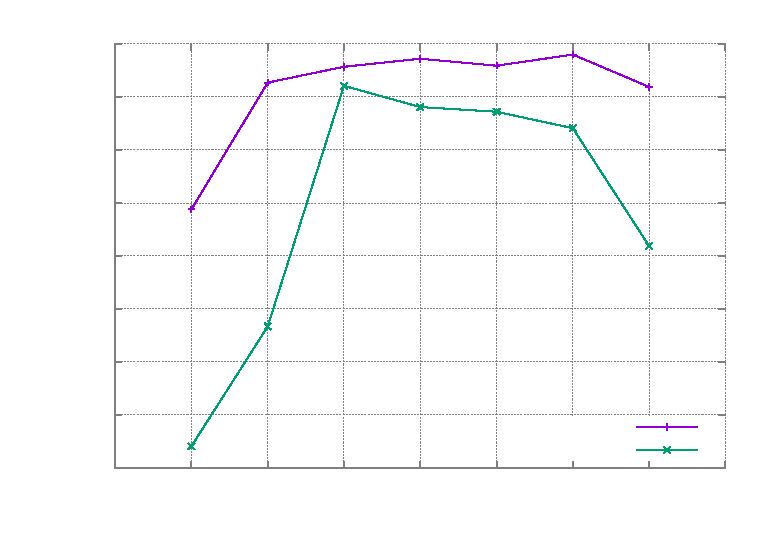
\includegraphics{grafovi/cnn_complexity}}%
    \gplfronttext
  \end{picture}%
\endgroup

    \caption{Usporedba 7 dubokih konvolucijskih arhitektura različitih kompleksnosti}
    \label{graf:cnncomplex}
\end{center}
\end{figure}

Kao i kod analize standarnih neuronskih mreža rezultati na sintetiziranom testnom skupu bolji su od onih na ručno označenom skupu, no za određene arhitekture ta je razlika vrlo mala. Na prikazu rezultata vidljiva je standarna krivulja generalizacije za oba testna skupa. Točnost klasifikacije je mala za nedovoljno kompleksne modele jer njihova arhitektura nema dovoljno slobodnih parametara da bi kvalitetno opisala podatke hijerarhijom značajki. Za pretjerano kompleksne modele je točnost na testnim skupovima također manja zbog previše slobodnih parametara koji omogućuju pretjeranu prilagođenost modela podatcima za učenje. Analizom je pronađena optimalna arhitektura sa 10 mapa značajki u prvom konvolucijskom sloju te 20 mapa značajki u drugom konvolucijskom sloju. Rezultati modela sa optimalnom arhitekturom pokazuju dobru sposobnost generalizacije na oba testna skupa.

\section{Usporedba optimalnih arhitektura}

Usporedbom najboljih predstavnika standarnih i konvolucijskih neuronskih mreža moguće je dobiti uvid u utjecaje različitih tipova arhitektura. Analizom standarnih mreža pokazano je da se dodavanjem dubine plitkoj dvoslojnoj mreži povećava njena sposobnost generalizacije. Optimalna konvolucijska arhitektura također je duboka, stoga dobiveni rezultati upućuju na prednost dubokih arhitektura nad plitkima. 

U Tablici \ref{tab:standconv} prikazana je usporedba rezultata dva optimalna modela na oba testna skupa. Točnost klasifikacije na sintetiziranom skupu približno je jednaka za oba modela, no na ručno označenom skupu rezultati su bolji kod konvolucijskog modela. Rezultati upućuju na to da konvolucijska arhitektura mreže poboljšava sposobnost generalizacije modela.  

\hspace{2em}
\begin{table}[ht!]
\begin{center}
\centering
    \begin{tabular}{ | c| c| c|c |}
    \hline    		
    Skup podataka & Standarna arhitektura & Konvolucijska arhitektura \\ \hline
    Sintetizirani & 99.91\% & 99.57\%  \\ \hline
    Ručno označeni & 96.31\% & 	99.21\%  \\
    \hline
    \end{tabular}
\end{center}
\caption{Usporedba standarnih i konvolucijskih arhitektura}
\label{tab:standconv}
\end{table}

Analizom točnosti klasifikacije za svaku zasebnu klasu te promatranjem krivo klasificiranih primjera mogu se točno vidjeti slučajevi koji standarnoj neuronskoj mreži predstavljaju problem, a koje konvolucijska neuronska mreža uspijeva točno klasificirati. U Tablici  \ref{tab:hardexample} prikazana je usporedba postotka točnosti klasifikacije za takve slučajeve. Jedan takav slučaj je sličnost između znamenke '0' i slova 'O' koji se razlikuju samo po zaobljenosti konture. Rezultati upućuju na to da lokalni filteri konvolucijskih mreža mogu robusnije predstaviti zaobljene konture i time doprinjeti robusnosti algoritma prilikom razlikovanja ovih klasa. Također problematičan slučaj predstavlja razlikovanje slova 'B' od znamenke '8'. Optimalni model standarne neuronske mreže velik broj slova 'B' krivo je klasificirao kao znamenku '8', dok je konvolucijska mreža imala vrlo visok postotak točnosti klasifikacije za obadvije klase.

\hspace{2em}
\begin{table}[ht!]
\begin{center}
\centering
    \begin{tabular}{ | c| c| c|c | c| c| c|}
    \hline    		
    Arhitektura & Znamenka '0' & Slovo 'O' & Znamenka '8' & Slovo 'B'  \\ \hline
    Standarna & 74.15\% & 91.97\% & 98.69\% & 38.57\%  \\ \hline
    Konvolucijska & 97.55\% & 95.35\% & 99.81\% & 99.29\%   \\
    \hline
    \end{tabular}
\end{center}
\caption{Usporedba arhitektura na teškim slučajevima}
\label{tab:hardexample}
\end{table}

Osim točnosti naučenih klasifikatora prilikom analize uzeta je u obzir i njihova kompleksnost te prosječno trajanje klasifikacije. Kao što je ranije spomenuto, kompleksnost modela može se aproksimirati preko broja računskih operacija potrebnih za klasifikaciju jedne slike, ili preko broja slobodnih parametara, odnosno broja težina koje se mogu mijenjati prilikom učenja mreže.  

\hspace{2em}
\begin{table}[ht!]
\begin{center}
\centering
    \begin{tabular}{ | c| c| c|c | c| c| c|}
    \hline    		
    Svojstvo & Standarna arhitektura & Konvolucijska arhitektura \\ \hline
    Broj računskih operacija & 170550 & 97780  \\ \hline
    Broj slobodnih parametara & 170550 & 6930   \\ \hline
    Prosječno trajanje klasifikacije  & 0.202 ms & 0.223 ms \\
    \hline
    \end{tabular}
\end{center}
\caption{Usporedba svojstava kompleksnosti arhitektura}
\label{tab:complexity}
\end{table}

U tablici \ref{tab:complexity} prikazana je usporedba navedenih svojstava za oba optimalna modela. Po broju računskih operacija standarni model gotovo je dvostruko kompleksniji, no prosječno trajanje klasifikacije približno je jednako za oba modela. Razlog tome je što se proječno trajanje klasifikacije računa empirijski te ovisi o implementaciji svih računskih operacija, koje u ovom slučaju traju dulje kod konvolucijskih mreža. 

Važno je primjetiti da konvolucijska arhitektura ima za red veličine manji broj slobodnih parametara od standarne arhitekture. Manji broj slobodnih parametara izravna je posljedica dodatnih ograničenja koja mehanizmi dubokih konvolucijskih mreža postavljaju na kompleksnost modela. Ovo svojstvo konvolucijskog modela doprinosi njegovoj sposobnosti generalizacije, te omogućuje u konačnici bolje rezultate na ručno označenom skupu podataka.

\section{Usporedba sa Microblink klasifikatorom}

Osim analize raznih arhitektura neuronskih mreža, u sklopu ovog rada provedena je i analiza internog klasifikatora tvrtke Microblink. Radi se o klasifikatoru razvijenom po klasičnim principima rješavanja problema raspoznavanja znakova gdje se klasifikacija provodi u tri glavna koraka. Prvi korak je predprocesiranje ulazne slike gdje se nastoji ublažiti transformacije nastale promjenjivim uvjetima okoline. Idući korak je računanje diskriminantnih značajki ulazne slike kako bi se dodatno olakšao problem klasifikacije, te je konačni korak primjena algoritma klasifikacije na značajkama slike.

\hspace{2em}
\begin{table}[ht!]
\begin{center}
\centering
    \begin{tabular}{ | c| c| c|c |}
    \hline    		
    Klasifikator & Sintetizirani skup  & Ručno označeni skup \\ \hline
    Microblink  & 86.93\% & 91.69\%  \\ \hline
    Standarna mreža & 99.91\% & 96.31\%  \\ \hline
    Konvolucijska mreža & 99.57\% &  99.21\% \\
    \hline
    \end{tabular}
\end{center}
\caption{Usporedba Microblink klasifikatora sa optimalnim neuronskim mrežama}
\label{tab:mbstandconv}
\end{table}

Usporedbom rezultata u Tablici \ref{tab:mbstandconv} može se vidjeti da interni klasifikator tvrtke Microblink daje lošije rezultate od standarnih i konvolucijskih neuronskih mreža.
Postoji više faktora koji u teoriji objašnjavaju ovakve rezultate. Jedan problem je negativni utjecaj predprocesiranja podataka zbog nesavršenosti ručno razvijenih metoda obrade slike. Zbog gubitka informacija neke od slika postaju neprepoznatljive nakon algoritma za predprocesiranje, što čini točnu klasifikaciju nemogućom. Još jedan faktor koji otežava klasifikaciju težih primjera je nesavršenost ručno definiranih značajki slike koje se predaju klasifikatoru. Umjesto da se značajke uče na temelju skupa podataka kako bi se maksimizirala njihova diskriminantnost, one se ručno definiraju na temelju ljudskog promatranja podataka što dovodi do gubitka informacija. Te konačno, ovako razvijeni klasifikator ima samo jedan sloj asptrakcije što onemogućuje stvaranje hijerarhije značajki koje robusnije predstavljaju objekt klasifikacije i poboljšavaju točnost klasifikatora.

\hspace{2em}
\begin{table}[ht!]
\begin{center}
\centering
    \begin{tabular}{ | c| c| c|c |}
    \hline    		
    Klasifikator & Prosječno trajanje klasifikacije \\ \hline
    Microblink & 0.025 ms \\ \hline
    Standarna mreža & 0.202 ms  \\ \hline
    Konvolucijska mreža &  0.223 ms \\
    \hline
    \end{tabular} 
\end{center}
\caption{Usporedba prosječnog trajanja klasifikacije}
\label{tab:avgduration}
\end{table}

Prednost Microblink klasifikatora u odnosu na odabrane modele neuronskih mreža je njegova brzina. U Tablici \ref{tab:avgduration} može se vidjeti da je njegovo prosječno trajanje klasifikacije za red veličine manje od onog od neuronskih mreža. Brzine neuronskih modela još uvijek su dovoljno velike za primjenu u stvarnom vremenu na mobilnom uređaju, no konačna brzina klasifikatora može se i dodatno smanjiti ukoliko se koriste u kombinaciji sa bržim Microblink klasifikatorom. 

\section{Moguća poboljšanja}
 
Kao i kod svakog pristupa, moguća su poboljšanja u točnosti i brzini izvođenja klasifikacije. U području dubokog učenja veliki je naglasak na učenju svakog koraka procesa klasifikacije na temelju podataka, stoga je dodatni naglasak na važnosti podataka za učenje. Predstavljene duboke konvolucijske arhitekture pokazale su se sposobnima graditi kvalitetne hijerarhije značajki na temelju podataka, no za to je prije svega potrebna velika količina kvalitetnih podataka koji dobro predstavljaju domenu problema. Stoga je za budući napredak prije svega potrebno prikupljanje što veće količine kvalitetnih podataka za učenje. 

Najbolji rezultati u ovom radu postignuti su sa konvolucijskom arhitekturom vrlo male kompleksnosti, svega nekoliko tisuća slobodnih parametara. Dodatnim povećavanjem kompleksnosti smanjivala se sposobnost generalizacije modela, što upućuje na pretjeranu prilagodbu podatcima za učenje. Ograničavanje kompleksnosti klasifikatora kako bi se povećala sposobnost generalizacije standarni je pristup prilikom selekcije modela, no pretjerana potreba za ovim metodama upućuje na nedovoljno kvalitetne podatke za učenje. Za učenje se u ovom radu koristi sintetizirani skup podataka prikupljen nad imitacijama osobnih iskaznica i u kontroliranim uvjetima. Stoga je jedno od mogućih poboljšanja razvijanje kvalitetnijih imitacija kartica, te porađivanje na raznolikosti uvjeta prilikom njihovog slikanja.

Naučeni duboki konvolucijski modeli tipično imaju vrlo malu brzinu izvođenja klasifikacije zbog njihove velike dubine i kompleknosti, što ih čini teže primjenjivima na problemima u stvarnom vremenu. U ovom radu optimalni modeli vrlo su male kompleknosti zbog ranije spomenutih razloga, te imaju dovoljno veliku brzinu izvođenja klasifikacije za primjenu u stvarnom vremenu. No poboljšavanjem kvalitete podataka za učenje moći će se iskoristiti potencijal kompleksnijih modela, što će za posljedicu imati problem izvođenja tih modela u stvarnom vremenu. Jedna metoda koja bi mogla poboljšati brzinu ovakvih modela je metoda Geoffreya Hintona pod nazivom distilacija \engl{Distillation}\cite{hinton2015distill}. Ideja je koristiti izlaze naučenog velikog modela kao takozvane mekane oznake za svaku sliku prilikom učenja manjeg modela. Istraživanje je pokazalo da se sa mekanim oznakama prenosi dio informacija o podatcima koje je prikupio veliki model, što poboljšava konačnu točnost naučenog manjeg modela. Tako naučeni manji model može se koristiti u stvarnom vremenu zbog svoje manje kompleksnosti i time veće brzine izvođenja klasifikacije.   



\chapter{Zaključak}

Prepoznavanje teksta sa slike ima vrlo široku primjenu u mnogim područjima ljudske djelatnosti. Razvijanjem mobilne tehnologije pojavljuju se nove izazovnije primjene optičkog prepoznavanja znakova. Algoritam za prepoznavanje znakova mora biti robustan na promjenjive uvjete okoline, ali i dovoljno brz za primjenu u stvarnom vremenu na mobilnim uređajima. 

Duboko učenje je novo obečavajuće područje istraživanja inspirirano vizualnim korteksom mozga sisavca. Zasniva se na učenju korisnih prezentacija podataka povezanih u obliku hijerarhije, te je pokazalo jako dobre rezultate na problemima raspoznavanja uzoraka. Za problem klasifikacije u računalnom vidu razvijene su duboke konvolucijske neuronske mreže koje traže lokalne značajke na slici pomoću lokalnih filtera ostvarenih konvolucijom. 

U ovom radu razvijen je sustav za učenje i testiranje različitih arhitektura neuronskih mreža, kao i prikaz rezultata u svrhu usporedbe različitih modela. Korištenjem sustava provedeno je istraživanje primjene standarnih neuronskih mreža i dubokih konvolucijskih neuronskih mreža na problemu raspoznavanja znakova. Rezultati su prikazani i komentirani sa ciljem pronalaska optimalne arhitekture modela za primjenu na mobilnom uređaju, a osim točnosti naučenih klasifikatora uzeta je u obzir i njihova kompleksnost te prosječno trajanje klasifikacije. Također je razvijeno sučelje za korištenje naučenih modela mreža kao klasifikatora u Microblink OCR sustavu čime je omogućena dodatna analiza primjenom modela na mobilnom uređaju.

Dobiveni rezultati potvrdili su prednosti primjene dubokih konvolucijskih mreža na problemu raspoznavanja znakova. 

Analiziranjem rada klasifikatora sa i bez predprocesiranja podataka pokazana je prednost prosljeđivanja neobrađenih slika klasifikatoru u svrhu očuvanja informacija slike. Posljedice promjenjivih uvjeta okoline se tada rješavaju na način da se procesom učenja na velikoj količini različitih oblika podataka razvije kvalitetna hijerarhija značajki otporna na nastale transformacije.

Postupkom selekcije modela nad standarnim neuronskim arhitekturama ustanovljeno je da se dodavanjem dubine neuronskoj mreži pospješuje njena sposobnost generalizacije. Ovaj rezultat može se protumačiti kao posljedica razvijanja hijerarhije značajki koja robusnije predstavlja objekt detekcije. 

Usporedbom rezultata optimalnih modela standarnih i konvolucijskih neuronskih mreža pokazana je prednost korištenja konvolucijske arhitekture na problemu raspoznavanja znakova. Konvolucijska arhitektura ima za red veličine manji broj slobodnih parametara od standarne arhitekture, što je izravna posljedica dodatnih ograničenja koje mehanizmi dubokih konvolucijskih mreža postavljaju na kompleksnost modela. To svojstvo konvolucijskog modela doprinosi njegovoj sposobnosti generalizacije, te omogućuje u konačnici bolje rezultate na ručno označenom skupu podataka.

Rezultati klasifikatora tvrtke Microblink lošiji su od rezultata standarnih i konvolucijskih neuronskih mreža, što se može objasniti negativnim utjecajem predprocesiranja podataka i ručnog definiranja značajki samo jedne razine apstrakcije. Prednost Microblink klasifikatora u odnosu na odabrane modele neuronskih mreža je njegova za red veličine veća brzina, no brzine neuronskih modela još uvijek su dovoljno velike za primjenu u stvarnom vremenu na mobilnom uređaju. 

\bibliography{literatura}
\bibliographystyle{fer}

\begin{sazetak}

U ovom radu provedeno je istraživanje primjene dubokih konvolucijskih neuronskih mreža na problemu raspoznavanja znakova. U tu svrhu razvijen je sustav za učenje i testiranje različitih arhitektura neuronskih mreža. Podsustav za učenje implementiran je pomoću razvojnog alata za paralelno računanje na grafičkoj kartici kako bi postupak bio što brži. Dio sustava za testiranje razvijen je s ciljem detaljne analize rada naučenih modela, te jednostavne i pregledne usporedbe više različitih modela. 

Istraživanje je ostvareno uz dodatnu podršku tvrtke Microblink specijalizirane za razvoj tehnologija računalnog vida za mobilne uređaje. Za učenje i testiranje modela koriste se od tvrtke interni skupovi podataka, a prilikom testiranja provodi se analiza i njihovog internog klasifikatora. 
Rezultati su prikazani i komentirani sa ciljem pronalaska optimalne arhitekture modela za primjenu na mobilnom uređaju. Pritom je osim točnosti naučenih klasifikatora uzeta u obzir i njihova kompleksnost te prosječno trajanje klasifikacije.

\kljucnerijeci{računalni vid, raspoznavanje znakova, neuronske mreže, duboko učenje, konvolucijske mreže}
\end{sazetak}

\newpage

\engtitle{Deep convolutional neural networks for character recognition}
\begin{abstract}

In this thesis, deep convolutional neural networks for optical character recognition have been researched. For this purpose a system for learning and testing of different architectures of neural networks has been developed. Subsystem for learning was implemented with development tools for parallel computing on graphics cards to make the procedure as fast as possible. Part of the system for testing was developed for detailed analysis of the learned models, as well as simple and transparent comparison of different models.

The research had additional support from the company Microblink specialized in the development of computer vision technology for mobile devices. Internal datasets from the company are used for the learning and testing of models, and additional analysis was conducted on the companies internal classifier.
The results are presented and discussed with the aim of finding the optimal model architecture for the application on a mobile device. In addition to the accuracy of the learned classifiers, their complexity and average classification duration was taken into account as well.

\keywords{computer vision, character recognition, neural networks, deep learning, convolutional networks}
\end{abstract}

\end{document}
